\documentclass[12pt,a4paper]{ctexart}
\usepackage{amsmath,amssymb,bm}
\usepackage{graphicx}
\graphicspath{{figures/}}
\usepackage{booktabs}
\usepackage{longtable}
\usepackage{array}
\usepackage{geometry}
\usepackage{caption}
\usepackage{float}
\usepackage{needspace}
\usepackage[hidelinks]{hyperref}
\geometry{left=2.5cm,right=2.5cm,top=2.5cm,bottom=2.5cm}
\captionsetup[figure]{labelsep=space,font=small}
\captionsetup[table]{labelsep=space,font=small}
\newcolumntype{C}[1]{>{\centering\arraybackslash}p{#1}}
\setlength{\parindent}{2em}
\linespread{1.08}
\renewcommand{\arraystretch}{1.2}
\title{论文3}
\date{}
\setCJKfamilyfont{hei}[AutoFakeBold=2]{SimHei}
\ctexset{section={format=\heiti\bfseries\zihao{4},beforeskip=10pt,afterskip=6pt},subsection={format=\heiti\bfseries\zihao{-4},beforeskip=8pt,afterskip=4pt},subsubsection={format=\heiti\bfseries\zihao{-4},beforeskip=6pt,afterskip=3pt}}
\begin{document}
\setlength{\abovedisplayskip}{6pt}
\setlength{\belowdisplayskip}{6pt}

\begin{center}\Large\bfseries 微网购电与储能调度的分期决策模型\end{center}

\begin{center}\Large\bfseries 摘 要\end{center}

针对光伏出力、负荷及电价变化下的微网购电与储能调度，本文建立预测、风险储备、计划决策与实际执行相衔接的模型，在满足电量守恒、储能容量与功率限制的条件下控制购电费用。全年跨日连续运行，1月为预热期，2月至12月共334天为正式评价期。

问题一采用单日线性规划，并设置首尾储电量相等的日循环约束。HiGHS求得全天购电量59,482.6990 kWh、购电费35,126.9486元；充放电量之比为0.810000，与往返效率一致。

问题二集成近期基线、岭回归与LightGBM预测负荷和光伏，以历史累计净负荷残差估计安全储备，事前统一取启发式分位数0.80。日前计划采用线性规划，执行采用36段滚动MPC。正式期总费用13,864,639.36元，紧急购电量136,727 kWh，占负载0.369\%。

问题三在0、6、12、18时更新输入并重新决策：光伏输入融合附件3官方预报与自建预测，负荷输入根据已观测值作日内水平修正。按路径最小承诺结算的解释假设构造链式费用，修订阶段采用混合整数线性规划，执行采用贪心规则。正式期费用13,439,044.37元，比问题二低42.56万元；这一差额为不同配置的综合影响，不能单独归因于调整机制。

问题四增加历史信息驱动的电价预测，决策使用预测价格，结算使用实际价格。问题4-2、4-3正式期费用分别为14,595,194.94元和14,158,125.73元。发布时点消融显示正式期关闭6时可降低费用，但问题4-3在365天口径下反而多花10,448.05元，故保留完整配置作为正式基线。

全年轨迹通过电量守恒、SOC范围、功率上限与充放互斥核验；全知阶梯与分位数扫描用于界定信息差距和参数敏感性，不构成年度最优性或模块因果贡献的证明。各项费用与冻结输出一致。

关键词：微网调度；储能优化；线性规划；混合整数线性规划；风险储备；滚动预测控制

\clearpage

\needspace{4\baselineskip}\section*{一、问题重述}

微网是为促进光伏等分布式电源就地消纳、减轻并网压力而发展起来的小型发用电系统，光伏系统接入配电网的技术背景见文献\textsuperscript{[1]}。出于经济性考虑，非孤岛式微网可在电价较低或分布式电源有剩余电量的时段为储能设备充电，并在电价较高时段释放电能，从而在满足小区负载需求的同时尽可能节省购电费用；其调控的核心是依据小区负载、光伏发电功率与储能设备当前储电量，制定微网的购电量与储能设备的充放电量。

已知储能设备最大容量为 12000 kWh、最大充放电功率为 5000 kW，运行中电量须维持在 1200～10800 kWh 之间，充放电效率为 90\%，2025 年 1 月 1 日 0:00 的初始储电量为 6000 kWh。附件给出某典型日及 2025 年全年的电价、小区负载、光伏发电实际功率与预报功率等数据（时间粒度为 10 分钟）。据此，需解决以下四个问题：

问题 1：若每天电价与小区负载相同，且已知一天的光伏发电功率预测数据，在微网供给电能不低于小区负载、储能设备 0:00 与 24:00 储电量相同的前提下，建立每天 0:00 制定当日计划购电策略的数学模型，给出指定时段及全天的购电量与购电费、储能设备在各时段的充放电量与首末储电量。

问题 2：若每天电价相同而小区负载与光伏随时间变化，微网供电不足时须按交易时刻电价的 5 倍向外网紧急购电，建立每天 0:00 的当日计划购电策略模型，给出指定日期的购电、充放电及紧急购电结果。

问题 3：在每天 0:00、6:00、12:00、18:00 可获得未来 24 小时光伏发电功率预报的条件下，允许在非零时刻调整购电策略（计划量高于调整部分按交易电价的 50\% 计违约费，调整高于计划部分按 1.5 倍计价），建立微网当日购电策略的滚动优化模型，给出指定日期的结果，并分析是否需要引入其他时刻的预报来调整购电策略。

问题 4：针对外网电价实时波动的情形，建立波动电价下微网当日购电策略的数学模型，并重新求解问题 2 与问题 3，给出相应结果。

\needspace{4\baselineskip}\section*{二、问题分析}

\needspace{3\baselineskip}\subsection*{2.1 问题一的分析}

问题一在信息完全确定的条件下，要求每天 0:00 一次性给出全天 144 个时段的购电量与储能充放电量，本质是单周期确定性时序调度问题，核心机理是储能如何在峰谷电价之间搬运电量，其模型骨架可被后三问直接沿用。逐时段须确定购电量、充电量与放电量三个决策量，并与光伏出力、小区负载满足功率平衡；题目只允许电量由外网流入微网、不允许售电，因此购电量非负，富余光伏也不能倒送电网，只能充入储能或弃掉，故在平衡式中留出一个弃光出口（本算例中该出口未被启用，保留只为模型完备）。储能侧受四条约束支配：充放电功率均不超过 5000 kW；储电量全程落在 1200～10800 kWh 之内；充电与放电效率各为0.90，即从电网取入1 kWh经完整充放循环可送回0.81 kWh；以及 0:00 与 24:00 储电量相同、即日循环边界条件。以全天购电费用最小为目标，目标与约束对决策变量均为线性，故问题一归结为标准线性规划；又因往返效率小于 1，同时充放会增加能量损耗，本算例的求解结果满足充放互斥。需要说明的是，不能仅凭效率损耗断言任意最优解都互斥；后三问取消日循环硬约束并采用终端水值，其互斥性由逐时段可行性核验确认（见 6.1 节）。

\needspace{3\baselineskip}\subsection*{2.2 问题二的分析}

与问题一相比，问题二有两处本质变化：电价每天相同而小区负载与光伏逐日变化，且当天真实值在制定计划时并不可知，计划购电量不能再由当天净负荷直接推出；同时微网供电不足时缺口须按交易时刻电价的 5 倍紧急采购，而计划购电量无论是否用完均按原价结算，由此引入明显不对称的损失结构。不对称性决定了最优计划应当偏保守的幅度：计划量每少买 1 kWh，缺口要多支出 4 倍电价；每多买 1 kWh 而无用，只损失 1 倍电价。由报童模型的临界比 4$:$1 可得启示性分位数 0.80，本文据此在四个决策时刻统一取该值；但储能本身是一层缓冲，安全余量必须与储能调度联合确定，无储能的报童解不能直接照搬，0.80 在本模型中只是事前统一的启发式设置，其实际效果由 6.3 节的灵敏度扫描与覆盖率统计共同报告。因果性是本问的硬约束：当天 0:00 只能用该日之前的历史实际值，当天的实际值须待日末才并入历史库，否则会出现用当天真值反推计划量的信息泄露。已有家庭微网研究将供需不确定性纳入能量管理，并比较预测控制与随机控制方法\textsuperscript{[2]}。据此建立「预测—风险—决策—执行」四层模型，四层之间以净负荷预测与安全储备为接口，职责清晰且可分别检验。

\needspace{3\baselineskip}\subsection*{2.3 问题三的分析}

问题三的物理结构与问题二相同，变化来自输入信息与决策结算规则两方面：一天不再只做一次计划，而是允许在 0:00、6:00、12:00、18:00 四个时刻各修订一次购电承诺，且每次修订只能覆盖尚未执行的计划段；费用也不再是「计划量乘电价」的简单求和，而是链式结算——相对上一次已发布承诺上调的部分按 1.5 倍电价计超购费、下调的部分按 0.5 倍电价计违约费，各版本承诺中的最低一档构成结算基准量并按正常电价计基准费。由此产生两个难点：其一是路径依赖，历史最低承诺是随修订逐步下移的状态量，一次下调虽当期为承诺量省了钱，却把基准量永久压低，日后调回须按 1.5 倍补缴，故任一时刻的最优调整都不能孤立地看当期；其二是目标函数的分段非线性，上调、下调与基准量变化三段分别按 1.5、0.5、1.0 倍计价，含最大最小运算，决策层于是由线性规划变为混合整数线性规划。

与问题二的差别不止于决策层。预测层需要接入附件 3 各发布时刻的光伏预报并按时间对齐后与自有预测融合；风险层虽然仍取分位数 0.80，但误差样本的统计口径由「全天累计」改为「各决策时刻剩余窗口内的累计」，四个时刻各自统计；执行层由 36 段滚动 MPC 改为逐时段无前瞻贪心充放电规则。因此本文把它作为一套独立的「分阶段预测—分阶段储备—链式决策—贪心执行」配置处理，沿用问题二的物理约束与紧急购电费率，不宣称两问的预测层或执行层相同。

\needspace{3\baselineskip}\subsection*{2.4 问题四的分析}

问题四把外网电价由附件 1 的固定日内曲线换成附件 4 的逐日逐时段波动电价，并在新价格下重解问题二与问题三，得到 4-2 与 4-3 两个子问题；物理约束、储能参数与费用规则一律不变，唯一的新输入是价格信号本身。波动电价带来两点新困难：其一是电价由已知变为未知，当天 0:00 只能依据历史电价预测当日各时段价格，决策目标中出现的是预测电价而最终费用必须按实际电价结算，两支价格一旦混用就会得到现实中无法实现的费用；其二是跨日套利空间的出现，附件 4 的全年均价与附件 1 相同，说明价格被重新分配到不同时点，日间漂移使「低价日多买、高价日少买」成为新的收益来源，储能的角色由日内峰谷搬运扩展到日间搬运。据此，问题四沿用问题二的四层骨架，只在两处扩展：预测层增加一路电价预测，并规定决策目标一律用预测电价、费用恒等式一律用实际电价；决策层按子问题分岔，4-2 保持一次性日前线性规划与 36 段 MPC 执行，4-3 沿用链式混合整数规划与贪心执行。风险层统一采用事前分位数 0.80，但储备量由各自预测残差决定：问题 4-2 沿用问题二的储备规则，问题 4-3 沿用问题三各发布时点的储备规则。统一分位数并不意味着两个子问题的储备量相同；横向费用比较同时涉及预测、决策与执行配置的差异。

\begin{figure}[H]
\centering

\includegraphics[width=0.90\textwidth,height=0.55\textheight,keepaspectratio]{fig01.png}
\caption*{图1 问题建模和解决思路}
\end{figure}

\needspace{4\baselineskip}\section*{三、模型假设}

（1）平稳性假设：评价期内无重大政策调整与突发灾害等强外部冲击，电价曲线的日内形态、居民负载与光伏出力的季节规律保持稳定，不出现结构性跳变，从而由历史数据刻画的预测关系在评价期内仍然成立。

（2）储能简化假设：储能不随静置时间自放电，荷电状态仅由充放电量决定；充电与放电的单程效率均为 0.90，且不随功率大小、温度与循环次数变化，即往返效率恒为 0.81。

（3）外网交互假设：微网与外网之间的交换功率不受容量限制，缺电时必能以交易时刻电价的 5 倍即时购得所需电量；题目不允许向电网售电，富余光伏只能充入储能或弃掉。

（4）预测误差假设：净负荷预测误差的日内分布随时间平缓变化，可用历史残差的经验分布刻画；四个决策时刻各按自身剩余窗口内的累计残差统计储备，不假定四者分布相同。

（5）结算口径假设：罚则与费率（下调 0.5 倍、上调 1.5 倍、紧急购电 5 倍）直接取自题面；当同一天存在多次承诺时，各版本如何合成计费在题面中没有唯一说明，本文采用项目声明的一种解释假设——以各版本承诺的逐时段最小值为结算基准量、按正常电价计基准费，并对相邻版本之差分别计下调费与上调费。本文无官方答疑文件可供引用，该假设与实际结算规则的一致性未获外部验证。

（6）评价期假设：2025 年 1 月 1 日初始储电量取题面给定的 6000 kWh，此后跨日连续递推，1 月 1 日至 1 月 31 日为预热期，仅用于积累历史残差与递推储能状态，不计入费用统计；2 月 1 日不重新初始化储能状态。2 月 1 日至 12 月 31 日共 334 天为正式评价期，本文同时报告 2025 自然年 365 天口径的结果。问题二至问题四不设每日 0:00 与 24:00 储电量相等的硬约束——这是题面只对问题一提出的要求——改以日末储电量水值衔接相邻日期，另\textbf{由本文自行设定}年末储电量回到 6000 kWh 的收口条件，使跨问题的费用可比。题面本身未对问题二至问题四规定年末储电量目标。

\needspace{4\baselineskip}\section*{四、符号说明}

全文统一使用功率与电量两种量纲：负荷、光伏出力、购电及充放电的逐时段变量以 kW 计，储电量与风险储备以 kWh 计。每段电量等于该段平均功率乘以 $\Delta t=1/6$ h，费用中的功率变量只乘一次 $\Delta t$。程序的购电、充放电和弃光数组以每段电量存储，转换为本文功率变量时须除以 $\Delta t$。

问题一使用单日物理段下标 $i$。问题二至问题四区分自然日物理轴 $i$ 与计划轴 $j$：物理段 $i=1$ 为当日 00:00—00:10，计划段 $j=1$ 为当日 00:10—00:20，计划段 $j=144$ 为次日 00:00—00:10；两轴经 $\pi$ 与 $\psi$ 配对。历史日期统一记为 $\ell<d$，不再用 $j$ 同时表示历史日期。计划变量使用下标 $j$，实际执行与结算变量使用下标 $i$；带波浪号的输入表示按计划窗口重排后的预测或价格。

表1 本文的符号说明

{\fontsize{9.5}{11.5}\selectfont
\begin{longtable}{C{\dimexpr0.200000\textwidth-2\tabcolsep\relax}C{\dimexpr0.600000\textwidth-2\tabcolsep\relax}C{\dimexpr0.200000\textwidth-2\tabcolsep\relax}}
\caption*{表1 本文的符号说明}\\
\toprule
\textbf{符号} & \textbf{说明} & \textbf{单位} \\
\midrule
\endfirsthead
\toprule
\textbf{符号} & \textbf{说明} & \textbf{单位} \\
\midrule
\endhead
$d,\ell,D$ & 当前日期序号、历史日期序号及全年天数；$\ell<d$，$D=365$ & — \\
$i,j,T$ & 自然日物理段、计划段及每个完整日的段数；$T=144$ & — \\
$\pi(d,j)$ & 计划段到物理段：$j<T$ 时为 $(d,j+1)$，$j=T$ 时为 $(d+1,1)$ & — \\
$\psi(d,i)$ & 物理段到计划段：$i=1$ 时为 $(d-1,T)$，$i\ge2$ 时为 $(d,i-1)$ & — \\
$\Delta t$ & 每段时长，$\Delta t=1/6$ & h \\
$\mathcal K,J_k,I_k$ & 发布小时集合 $\mathcal K=\{0,6,12,18\}$、计划决策窗口及当日物理残差窗口 & — \\
$c_i,c_{d,i},\widehat c_{d,i}$ & 固定电价、实际波动电价及由历史数据生成的预测电价 & 元/kWh \\
$\widetilde c_{d,j}^{\mathrm{dec}}$ & 计划窗口的决策电价；固定价按窗口重排，波动价用预测值，尾段延续当日首段值 & 元/kWh \\
$L_{d,i},P_{d,i}^{\mathrm{act}}$ & 实际负荷与实际光伏功率 & kW \\
$L_{d,i}^{\mathrm{raw}},P_{d,i}^{\mathrm{raw}}$ & 集成模型水平校正前的输出 & kW \\
$L_{d,i}^{\mathrm{own}},P_{d,i}^{\mathrm{own}}$ & 自建模型的日前基础预测；不表示官方预报 & kW \\
$P_{d,i}^{(k)}$ & 附件3在 $k$ 时发布、经十分钟对齐后的官方光伏预报 & kW \\
$L_{d,i}^{\mathrm{fc},(k)},P_{d,i}^{\mathrm{fc},(k)}$ & 发布时刻 $k$ 的负荷预测与最终光伏预测；问题三光伏为融合结果 & kW \\
$\widetilde L_{d,j}^{\mathrm{fc},(k)},\widetilde P_{d,j}^{\mathrm{fc},(k)}$ & 对应计划窗口的预测输入；末段负荷延续当日首段预测，光伏取零 & kW \\
$E_{d,i}^{\mathrm{act}}$ & 自然日物理段末实际储电量，$E_{d,0}^{\mathrm{act}}$ 为午夜状态 & kWh \\
$E_{d,j}^{\mathrm{plan},(k)}$ & 发布时刻 $k$ 的计划段末储电量；省略 $(k)$ 时指首次计划 & kWh \\
$E_0,E_{\min},E_{\max}$ & 初始储电量6000、运行下限1200、运行上限10800；额定容量12000 & kWh \\
$P_{st}^{\max},\eta_c,\eta_d$ & 最大充放电功率5000 kW；充电与放电效率均为0.90 & kW；—；— \\
$x_{d,j},x_{d,j}^{(k)}$ & 首次计划及发布时刻 $k$ 后的承诺购电功率；未覆盖段沿用上一版 & kW \\
$x_{d,j}^{*},k^*(j)$ & 计划段的最终生效承诺及其最后可修订时刻，$k^*(j)=\max\{k\in\mathcal K:j\in J_k\}$ & kW；— \\
$\bar x_{d,i}^{(k)},x_{d,i}^{\mathrm{exec}}$ & 各版承诺经 $\psi$ 映射到物理轴后的功率及实际生效承诺；$x_{d,i}^{\mathrm{exec}}=x_{\psi(d,i)}^*$ & kW \\
$y_{d,i},r_{d,i}$ & 实际使用的承诺功率及未用功率，$r_{d,i}=x_{d,i}^{\mathrm{exec}}-y_{d,i}$ & kW \\
$g_{d,i},w_{d,i},e_{d,i}$ & 实际使用光伏、实际弃光及紧急购电功率 & kW \\
$u_{d,i},v_{d,i}$ & 实际充电与放电功率；计划量另记 $u_{d,j}^{\mathrm{plan}},v_{d,j}^{\mathrm{plan}}$ & kW \\
$w_{d,j}^{\mathrm{plan}}$ & 计划平衡中的富余功率出口，可包含未用购电与弃光 & kW \\
$\Delta_{d,j}^{\pm(k)},\bar\Delta_{d,i}^{\pm(k)}$ & 计划轴的上调、下调功率及映射到物理轴后的对应量；未覆盖段取零 & kW \\
$m_{d,j}^{(k-)}$ & 本次修订前各版承诺的历史最低功率 & kW \\
$y_{d,i}^{\mathrm{base}}$ & 结算基准功率，$y_{d,i}^{\mathrm{base}}=\min_{k\in\mathcal K}\bar x_{d,i}^{(k)}$；与实际使用量 $y_{d,i}$ 区分 & kW \\
$C_d,C$ & 实际日总费用及评价期总费用；不含终端水值 & 元 \\
$C_d^{\mathrm{grid}}$ & 基准购电费用 & 元 \\
$C_d^{\mathrm{adj}},C_d^{\mathrm{emer}}$ & 调整购电费及紧急购电费 & 元 \\
$\lambda_E,\bar c^{\mathrm{dec}}$ & 终端储电量价值系数及窗口决策电价均值，$\lambda_E=\eta_d\bar c^{\mathrm{dec}}$ & 元/kWh \\
$N_{d,i},N_{d,i}^{\mathrm{act}},\xi_{\ell,i}$ & 预测净负荷、实际净负荷及历史预测误差；分时发布时增加上标 $(k)$ & kW \\
$R_d,\widehat R_d,R_d^{(k)}$ & 原始残差分位数、内核有效储备及分时发布的原始储备 & kWh \\
$q,Q_q$ & 储备分位数及经验分位数算子；正式设置 $q=0.80$ & — \\
$W_d$ & 仅由历史信息估计的光伏有效发电物理段集合 & — \\
$\lambda_d,\rho_\ell,\omega_{d,\ell}$ & 日前水平因子、历史日电量比及衰减权重 & — \\
$n,\kappa,H_d$ & 水平校正有效样本数、收缩系数及历史样本日期集合 & — \\
$\rho_d^{(k)},\lambda_d^{(k)}$ & 已执行负荷的水平比及剩余段的阻尼修正系数 & — \\
$a_{d,k,h},b_{d,k,h}$ & 小时 $h$ 的光伏融合回归系数，不强制非负或和为1 & — \\
$\delta_{d,k,h}$ & 对应小时的融合回归截距 & kW \\
$\Delta F_{d,j}^{(k)},z,p,m$ & 修订费用增量与该计划段的新承诺、上一承诺、历史最低承诺 & 元；kW；kW；kW \\
$\mu,b^{\mathrm{bin}},M$ & 线性化辅助功率、二进制分支变量及松弛功率常数；$M=6.0\times10^5$ kW & kW；—；kW \\
$s_{d,i}$ & 实际供需余量，$s_{d,i}=x_{d,i}^{\mathrm{exec}}+P_{d,i}^{\mathrm{act}}-L_{d,i}$ & kW \\
\bottomrule
\end{longtable}
{\footnotesize\par\vspace{2pt}注：问题一省略日期及实际上标，所有下标 $i$ 均在单日物理轴上。问题二至问题四的计划量与物理量须先映射再配对。代码的 big-M 为每段电量 $10^5$ kWh，对应本文功率常数 $6\times10^5$ kW。$[a]^+=\max\{a,0\}$；$\operatorname{clip}(a,l,u)=\min\{u,\max\{l,a\}\}$。\par}
}

\needspace{4\baselineskip}\section*{五、模型建立与求解}

\needspace{3\baselineskip}\subsection*{5.1 问题一模型的建立与求解}

\subsubsection*{5.1.1 数据预处理}

附件 1 给出典型日 144 个 10 分钟时段的时间、电价、小区负载预测功率与光伏发电预测功率四列数据，无缺失值、无重复行。预处理主要解决时间列的口径问题。

其一是存储类型混用。发现 Excel 真时间数值（0:10—10:00）与纯文本（10:10—23:50，末行写作 0:00+1），两者不能直接比较或排序。统一折算为「距 0 点的分钟数」后得到 10、20、…、1440 共 144 个点，间隔恒为 10 分钟，无重复、无缺口。

其二是时间标签口径。附件 1、2、4 的时刻标签应理解为该 10 分钟物理段的结束时刻：首行代表 00:00—00:10，末行（即次日 00:00）代表 23:50—24:00，全天首尾闭合；本文把该轴称为自然日物理轴，段序号记作 $i$。附件 5 的计划行另按一条从 00:10 起算的计划轴解释，段序号记作 $j$，两条轴相差一段，其口径差别与唯一映射见 5.2.1 节。

净负荷定义为负载减光伏，即 $N=L-P$。净负荷为正表示需外网购电或储能放电，为负表示光伏有剩余。附件 1 典型日的曲线形态合理：0:00—5:00 净负荷约等于负载（约 3500 kW），8:00—16:00 转负、12:00 前后最低约 −2100 kW，18:00 后重新接近负载（如图2 所示）。

\begin{figure}[H]
\centering

\includegraphics[width=0.90\textwidth,height=0.55\textheight,keepaspectratio]{fig02.png}
\caption*{图2 典型日小区负载、光伏发电及其净负荷功率曲线}
\end{figure}

\subsubsection*{5.1.2 经济调度模型的建立}

除上面问题分析中提到的部分外，建模中另有两处题面条件必须专门处理：题目只允许电量由外网流入微网，故购电量非负；题目未给出上网电价，富余光伏不能倒送电网，只能在功率平衡中留出一个弃光出口。由附件 1 可知，全天光伏出力超过小区负载的时段共 30 个，但最大净富余功率仅 2117.5 kW，小于储能 5000 kW 的最大充电功率，故该出口在最优解中并未启用（详见 5.1.3），保留它只为模型完备。

模型涉及的量分为决策变量与状态变量两类。逐时段需要独立决策的有五个：外网计划购电功率 $x_i$、实际使用的计划购电功率 $y_i$、储能充电功率 $u_i$、储能放电功率 $v_i$ 与光伏实际使用功率 $g_i$，下标 $i=1,2,\dots,T$ 表示自然日物理段序号，$T=144$。购电浪费功率 $r_i=x_i-y_i$ 与光伏浪费功率 $w_i=P_i-g_i$ 由上述变量确定，属辅助变量。状态变量为各时段末的储电量 $E_i$，计 $E_0$ 至 $E_{144}$ 共 145 个。约束方面，$x_i\ge0$，$0\le y_i\le x_i$，$0\le g_i\le P_i$，$w_i\ge0$，充放电功率均不超过额定值 $P_{st}^{\max}=5000$ kW，储电量全程落在 $[E_{\min},E_{\max}]=[1200,10800]$ kWh 内。储能参数取自题面：额定容量 12000 kWh，充放电效率 $\eta_c=\eta_d=0.90$。问题一不含紧急购电，故紧急购电功率 $e_i\equiv0$，相关费用项全部消失。

微网在问题一中的全部支出只有一项，即按计划购电量计价的外网购电费，故以全天购电费用最小为目标：

\begin{equation}
\min\ C=\sum_{i=1}^{T} c_i x_i \Delta t
\end{equation}

约束条件由功率平衡、光伏侧约束、电网侧约束、储能动态、储电量范围、充放电功率上限与日循环七部分构成。首先是功率平衡约束，逐时段要求微网的供、需两侧相等：

\begin{equation}
y_i+g_i+v_i=L_i+u_i,\qquad i=1,2,\dots,T
\end{equation}

光伏侧约束刻画光伏出力的两个出口。光伏既不允许上网，也不能凭空消失，其出力只能被使用或被浪费，故有

\begin{equation}
g_i+w_i=P_i,\qquad 0\le g_i\le P_i,\qquad w_i\ge0
\end{equation}

电网侧约束则刻画购电的单向性与计划—实际的从属关系。购电只进不出，且实际使用量不得超过计划量：

\begin{equation}
0\le y_i\le x_i,\qquad r_i=x_i-y_i\ge0
\end{equation}

储能动态约束按「存入扣充电损耗、取出计放电损耗」的电网侧口径递推：

\begin{equation}
E_i=E_{i-1}+\eta_c u_i \Delta t-\frac{v_i \Delta t}{\eta_d},\qquad i=1,2,\dots,T
\end{equation}

该式的含义是充电时只有 $\eta_c$ 的比例真正存入电池，放电时每放出 1 kWh 需从存量中取出 $1/\eta_d$ kWh，往返效率为 $\eta_c\eta_d=0.9\times0.9=0.81<1$。储电量范围、充放电功率上限与日循环约束分别为

\begin{equation}
E_{\min}\le E_i\le E_{\max},\qquad 0\le u_i\le P_{st}^{\max},\qquad 0\le v_i\le P_{st}^{\max}
\end{equation}

\begin{equation}
E_T=E_0
\end{equation}

式(7)对应题面「储能设备在 0:00 和 24:00 的储电量相同」的要求，是一个把首尾对齐的边界条件，其作用是避免储能通过耗尽初始电量虚假压低购电费用。该条件只规定首尾相等而未规定共同取值，共同值即初始储电量 $E_0=6000$ kWh。

该模型是标准线性规划\textsuperscript{[3]}\textsuperscript{[4]}。写成 $x_i,u_i,v_i,w_i,E_i$ 的简化形式时，可消去实际使用功率 $y_i,g_i$，仅保留非负富余出口；共 $4T$ 个功率变量及 $T+1$ 个储电量状态，初末状态固定。目标与约束均为线性，可由 HiGHS 求得全局最优。效率损耗有利于避免同时充放，但原先``同时减去较小者后再利用多余储电量''的论证未保证容量和终端边界，不能证明任意最优解必然互斥。本文不据此作一般性结论，而以本算例逐段核验中 $\min(u_i,v_i)=0$ 的结果确认实际解互斥，无须在该算例额外引入二进制变量。

此外，日循环约束还给出一个不依赖具体数据的等价形式。对储能递推式在全天求和并代入 $E_T=E_0$，可得

\begin{equation}
\eta_c\sum_{i=1}^{T}u_i \Delta t=\frac{1}{\eta_d}\sum_{i=1}^{T}v_i \Delta t \quad\Longrightarrow\quad \frac{\sum_{i}v_i \Delta t}{\sum_{i}u_i \Delta t}=\eta_c\eta_d=0.81
\end{equation}

当全天充电量大于零时，放电总量与充电总量之比等于往返效率0.81，可用于校验结果；若全天充放电量均为零，求和等式仍成立，但比值不定义。

\subsubsection*{5.1.3 问题一经济调度模型的求解}

由 5.1.2 的性质一，问题一是决策变量全部连续、目标与全部约束均为线性的标准线性规划，求解阶段无须借助启发式搜索：贪心规则依赖人工设定的电价阈值且不保证全局最优，动态规划须把连续的储电量状态离散化、精度与计算量相互牵制。本文把模型整理后交由HiGHS求解。代码另加 $10^{-6}\sum_i w_i$ 的微小弃光惩罚，系数单位元/kW；本算例最优弃光为零，购电费用与式(1)一致。

求解结果为：全天购电量 59,482.6990 kWh，购电费用 35,126.9486 元，平均购电价 0.5905 元/kWh。储能全天充电 20,740.6661 kWh、放电 16,799.9396 kWh，往返损耗 3,940.7266 kWh，恰为充电总量的 19.00\%；全天弃光电量为 0。

为说明储能在本问中的作用，以光伏优先供负载、富余电量全部弃掉、不配储能作为基准方案对比：基准方案的购电费为 48,052.0466 元，配置储能后降至 35,126.9486 元，节省 12,925.0980 元，降幅 26.90\%。全天放电总量与充电总量之比为 $0.810000$，恰等于往返效率 0.81，与式(8)由日循环约束推出的等价形式完全一致，构成对求解结果的第一重校核。

\begin{figure}[H]
\centering

\includegraphics[width=0.90\textwidth,height=0.55\textheight,keepaspectratio]{fig03.png}
\caption*{图3 问题一储能 SOC 轨迹与充放电功率}
\end{figure}

最优策略呈现清晰的谷充峰放、午间补电形态。凌晨 0:00—0:50 电价处于全天谷段（约 0.43 元/kWh），储能以 5000 kW 的额定功率满功率充电；5:00—6:00 再以约 833 kW 补充充电，使储电量在早峰到来前升至上限。6:00—9:00 电价升至 0.88—1.10 元/kWh，储能转为放电，功率自 3618 kW 逐段递减至 1767 kW。11:50—12:40 光伏出力进入全天高峰（峰值 7612.3 kW 出现在 12:10），净负荷转负，储能再次以 5000 kW 满功率充电，把本会富余的光伏电量存入电池。18:00—20:00 电价升至全天最高（1.25—1.35 元/kWh），储能放电功率升至约 4270 kW，全天最大放电功率 4293.9 kW 出现在 20:40。22:00—24:00 电价回落至谷段，储能又以 3333 kW、2000 kW 的功率充电，为次日循环作准备。全天 144 个时段中，储能充电 45 段、放电 37 段，其余 62 段不动作。

\subsubsection*{5.1.4 问题一结果的分析}

题目要求的指定时间段购电量、全天购电量与购电费、储能充放电量与首末储电量分别见表 2 与表 3。

\begin{table}[H]
\centering\fontsize{9.5}{11.5}\selectfont
\caption*{表2 微网在指定时间段的购电量及全天的购电量和购电费}
\begin{tabular}{C{\dimexpr0.166667\textwidth-2\tabcolsep\relax}C{\dimexpr0.166667\textwidth-2\tabcolsep\relax}C{\dimexpr0.166667\textwidth-2\tabcolsep\relax}C{\dimexpr0.166667\textwidth-2\tabcolsep\relax}C{\dimexpr0.166667\textwidth-2\tabcolsep\relax}C{\dimexpr0.166667\textwidth-2\tabcolsep\relax}}
\toprule
\textbf{时间段} & \textbf{购电量 / kWh} & \textbf{时间段} & \textbf{购电量 / kWh} & \textbf{时间段} & \textbf{购电量 / kWh} \\
\midrule
10:00—10:10 & 0 & 12:00—12:10 & 480.4124 & 14:00—14:10 & 0 \\
16:00—16:10 & 445.4317 & 18:00—18:10 & 531.8940 & 20:00—20:10 & 0 \\
全天购电量 / kWh & 59,482.699 & 全天购电费 / 元 & 35,126.9486 & — & — \\
\bottomrule
\end{tabular}
\end{table}

\begin{table}[H]
\centering\fontsize{9.5}{11.5}\selectfont
\caption*{表3 储能设备在指定时间段的充放电量及 0:00 和 24:00 的储电量}
\begin{tabular}{C{\dimexpr0.166667\textwidth-2\tabcolsep\relax}C{\dimexpr0.166667\textwidth-2\tabcolsep\relax}C{\dimexpr0.166667\textwidth-2\tabcolsep\relax}C{\dimexpr0.166667\textwidth-2\tabcolsep\relax}C{\dimexpr0.166667\textwidth-2\tabcolsep\relax}C{\dimexpr0.166667\textwidth-2\tabcolsep\relax}}
\toprule
\textbf{时间段} & \textbf{充电量 / kWh} & \textbf{放电量 / kWh} & \textbf{时间段} & \textbf{充电量 / kWh} & \textbf{放电量 / kWh} \\
\midrule
0:00—4:00 & 4,500 & 0 & 4:00—8:00 & 833.3333 & 6,365.8412 \\
8:00—12:00 & 4,787.9643 & 1,702.997 & 12:00—16:00 & 5,286.0532 & 91.1014 \\
16:00—20:00 & 0 & 5,780.1319 & 20:00—24:00 & 5,333.3333 & 2,859.8681 \\
0:00 储电量 / kWh & 6,000 & — & 24:00 储电量 / kWh & 6,000 & — \\
\bottomrule
\end{tabular}
{\footnotesize\par\vspace{2pt}注：本表为约束 A（固定）口径下的求解结果。\par}
\end{table}

由表 2、表 3 可见，全天购电与储能充放电的时段分布与 5.1.3 求得的最优策略一致。储电量在本算例中确实触达了容量边界：上界 10800 kWh 在 5:50—6:00 与 14:40—18:10 共 21 个时点被触达，下界 1200 kWh 在 20:50—22:00 共 8 个时点被触达，说明谷充峰放的力度已把储能可用容量用满，容量约束并非虚设。全天光伏出力超过小区负载的时段共 30 个，但最大净富余功率仅 2117.5 kW，小于 5000 kW 的充电功率上限，富余电量可全部充入储能，故全天弃光电量恒为 0。

\begin{figure}[H]
\centering

\includegraphics[width=0.90\textwidth,height=0.55\textheight,keepaspectratio]{fig04.png}
\caption*{图4 问题一购电量曲线}
\end{figure}

\needspace{3\baselineskip}\subsection*{5.2 问题二模型的建立与求解}

\subsubsection*{5.2.1 数据预处理与信息集划分}

问题二的数据基础与问题一有本质差别：附件 1 直接给出当天的负载与光伏预测功率，计划量可由当天的净负荷直接推出；本问则要求依据附件 1 的电价与附件 2 的实际数据，在每天 0:00 制定当天的计划购电策略。附件 2 为 365 天 $\times$ 144 个十分钟时段的小区负载与实际光伏功率，各含 52,560 个观测：负载 1995.72—7978.88 kW、全年均值 4626.03 kW，光伏 0—10216.20 kW、全年均值 2311.79 kW，均无缺失值、无重复日期、无时刻缺口。电价沿用附件 1 的 144 点单日曲线（最低 0.3713 元/kWh 于 5:30—5:40，最高 1.3952 元/kWh 于 20:30—20:40，均值 0.7662 元/kWh），在全年逐日重复；其峰谷价差正是分时电价机制下储能套利的直接来源\textsuperscript{[5]}。

时间轴口径与问题一不同：从本问起同时存在两条时间轴。附件 1、2、4 的实际数据按自然日物理轴 $i$ 解释，附件 5 的计划行按计划轴 $j$ 解释。两轴唯一映射为 $\pi(d,j)=(d,j+1)$（$j\le143$）与 $\pi(d,144)=(d+1,1)$，反向映射为 $\psi(d,i)=(d-1,144)$（$i=1$）与 $\psi(d,i)=(d,i-1)$（$i\ge2$），故自然日首个物理段执行的是前一计划日的第 144 段承诺。结算时必须先经反向映射配对，不得把计划数组与原始负载数组按相同列号直接相乘。

更关键的一步预处理是信息集划分。第 $d$ 天 0:00 制定计划时，只允许使用 $\ell<d$ 的历史实际值与电价曲线；第 $d$ 天的实际负载与实际光伏只在该日结束后才并入历史库，用于更新次日的预测与安全储备。实现上通过逐日前向回放保证——每天的预测、安全储备与线性规划都在同一时点完成，全程不引用任何未来信息。

评价期按上述口径划分为两段：2025 年 1 月 1 日至 1 月 31 日为预热期，仅用于积累历史残差与递推储电量状态，不计入费用统计；2025 年 2 月 1 日至 12 月 31 日为正式评价期，共 334 天。储能初值取题面给定的 1 月 1 日 0:00 电量 6000 kWh，此后跨日连续递推，2 月 1 日不重新初始化。首日为冷启动——1 月 1 日 00:00—00:10 无前一计划日的第 144 段承诺可执行，该段承诺量取零。末日为跨年截断：12 月 31 日计划行的第 144 段属 2026 年 1 月 1 日，该段计划保留输出，但不计入 2025 年的实际执行与费用。为与题目正式输出期对照，本文同时报告 365 天与 334 天两个口径的费用。

\subsubsection*{5.2.2 基于累计风险储备的日前购电模型的建立}

建模思路：问题二的决策本质是带不对称损失的日前随机决策。计划购电偏低时缺口须按交易时刻电价的 5 倍紧急采购，每少买 1 kWh 相对已付的计划电价多支出 $4c_i$；计划购电偏高时未被使用的部分仍按原价结算，每多买 1 kWh 损失 $c_i$。这一不对称决定了最优计划应当比预测净负荷略偏保守，而偏保守的幅度由预测误差的分布决定。问题二还额外给出了储能这一缓冲通道：储能既能在低价时段多买、高价时段少买，也能在预测偏差真正出现时临时放量。据此把模型分成四层：预测层给出净负荷点预测 $N_{d,i}$；风险层用历史预测误差的分布给出储能安全储备 $R_d$；决策层把 $R_d$ 作为储电量的下限送入确定性线性规划；执行层再按十分钟滚动安排储能放电。层间接口只有 $N_{d,i}$ 与 $R_d$ 两个量，职责清晰且可分别检验。

净负荷预测：对负载和光伏分别构造三类基学习器——近期加权基线、岭回归与浅层梯度提升树，其中梯度提升实现采用 LightGBM\textsuperscript{[6]}。输入只包含制定计划时可见的特征（1、2、7、14 日滞后值，同一时段近 3、7、14 日均值，日内周期编码、星期编码与年内日序编码，以及近期水平趋势）。三类模型的合成权重由其近期损失确定：近期损失取指数加权平均绝对误差与同期绝对误差 0.75 分位数的加权和（权重分别为 0.85 与 0.15），前者刻画平均精度、后者刻画尾部风险。训练窗长度随历史残差的漂移强度在 45—180 天之间自适应缩放：残差漂移剧烈时缩短窗口，以削弱季节切换时旧样本的干扰。

光伏出力具有「夜间必为零」的硬结构，纯回归输出会在清晨与黄昏产生虚假的小额出力，且随季节推移日出日落时刻不断变化。光伏预测综述讨论了数据驱动预测方法及其输入、预测时域等因素\textsuperscript{[7]}；本文依据夜间无光伏出力的物理结构，根据历史光伏序列中连续有效发电的区间估计第 $d$ 天的有效窗口 $W_d$，把窗口外的预测置零。此外，负载与光伏都存在缓慢的季节漂移，仅靠滞后特征难以完全跟上，故用历史实际日电量与基础预测日电量之比估计水平因子：

\begin{equation}
\lambda_d=\operatorname{clip}\left(1+\frac{n}{n+\kappa}\left[\frac{\sum_{\ell\in H_d}\omega_{d,\ell}\rho_\ell}{\sum_{\ell\in H_d}\omega_{d,\ell}}-1\right],0.85,1.15\right)
\end{equation}

其中 $H_d$ 是截至第 $d$ 日之前、最近水平校正窗口内的有效历史日期集合，$n=|H_d|$；$\rho_\ell$ 为实际日电量与基础预测日电量之比，$\omega_{d,\ell}$ 为随样本年龄指数衰减的权重，$\kappa$ 为收缩系数。$n=0$ 时取 $\lambda_d=1$。负荷与光伏各自估计该因子，$n/(n+\kappa)$ 使小样本时向1收缩，限幅操作将校正控制在$\pm$15\%。

\begin{equation}
L_{d,i}^{\mathrm{fc}}=\lambda_d^L L_{d,i}^{\mathrm{raw}},\qquad P_{d,i}^{\mathrm{fc}}=\lambda_d^P P_{d,i}^{\mathrm{raw}}\mathbf1(i\in W_d)
\end{equation}

净负荷预测为负载预测减光伏预测：

\begin{equation}
N_{d,i}=L_{d,i}^{\mathrm{fc}}-P_{d,i}^{\mathrm{fc}}
\end{equation}

它表示外部电网与储能需要共同承担的功率。净负荷允许为负，即光伏富余时段，在精度评价时不得把它裁剪为零。

安全储备：安全储备应由预测误差的分布决定，且只能由第 $d$ 天之前的历史估计。定义历史净负荷预测误差

\begin{equation}
\xi_{\ell,i}=\left(L_{\ell,i}-P_{\ell,i}^{\mathrm{act}}\right)-N_{\ell,i}
\end{equation}

即实际净负荷减预测净负荷；$\xi_{\ell,i}>0$ 表示实际净负荷高于预测，计划量偏少。储备统计采用自然日内已经完成的新计划可执行窗口：排除已由上一日承诺锁定的 00:00—00:10 段，只累计当日 00:10—24:00 的 143 段残差，不把计划窗口中的次日首段并入当天样本。第 $d$ 天只使用 $\ell<d$ 的样本，取累计残差电量的 80\% 分位数：

\begin{equation}
R_d=Q_{0.80}\left(\left\{\sum_{i=2}^{T}\xi_{\ell,i}\Delta t:\ \ell<d\right\}\right)
\end{equation}

分位数取 0.80 的依据是不对称边际损失之比 $4:1$。设缺口按 $5c_i$ 紧急采购，计划量每少买 1 kWh 相对已付计划电价多支出 $4c_i$；每多买 1 kWh 而未被使用，损失 $c_i$。使期望费用最小的临界分位数为

\begin{equation}
q^{*}=\frac{4c_i}{4c_i+c_i}=0.80
\end{equation}

式(14)是无储能单期报童模型的临界比结论，此处只借用其启发。本问的决策对象是一个带容量约束、跨时段耦合与效率损失的多阶段储能系统，其最优风险参数并无解析解，因此本文把 0.80 作为\textbf{事前统一的启发式设置}：它不含待估参数、不需要任何评价期数据，因而不存在以评价期结果反推风险参数的信息泄露问题；但它并不能被式(14)严格证明为多阶段系统的最优取值。其实际表现由 6.3 节的覆盖率统计与灵敏度扫描报告；日费用的尾部风险另用条件风险价值\textsuperscript{[8]}统计（见表 6 中的日费用 CVaR95）。

历史累计残差样本不足20天时取 $R_d=0$；否则用式(13)计算原始分位数。决策实际采用 $\widehat R_d=\min\{\max\{R_d,0\},4800\}$ kWh，原始分位数与有效储备不混写。为保证起始状态可达，令 $t_{\mathrm{lo}}=\lceil\max\{0,E_{\min}+\widehat R_d-E_{d,0}^{\mathrm{plan}}\}/(\eta_c P_{st}^{\max}\Delta t)\rceil$。代码以零号段为起点，从局部段号 $t_{\mathrm{lo}}$ 起施加储备下界；按本文从1起算的计划段号，该条件为 $j\ge t_{\mathrm{lo}}+1$：

\begin{equation}
E_{d,j}^{\mathrm{plan}}\ge E_{\min}+\widehat R_d\ (j\ge t_{\mathrm{lo}}+1),\qquad E_{\min}\le E_{d,j}^{\mathrm{plan}}\le E_{\max}
\end{equation}

需要强调的是，$\widehat{R}_d$ 随历史窗口滚动更新，是逐日变化的动态量，本文不存在「全年固定储备」的设定。同时，残差样本的经验覆盖率是「实际净负荷不超过预测净负荷加储备的样本比例」，它与「无紧急购电的概率」或「供电可靠率」不是同一个指标：即使储备覆盖了全部残差，只要储电量本身不足以支撑该缺口，仍会发生紧急购电。同理，日末储电量高于储备线也不足以证明当天储备约束全程不紧——该结论须逐时段核验储电量轨迹与储备线的关系后才能得出。

0:00的实际储电量记为 $E_{d,0}^{\mathrm{act}}$。当日首段承诺已由上一日尾段锁定，先用该承诺及当前可见的首段预测得到00:10的预测储电量，记为首次计划起点 $E_{d,0}^{\mathrm{plan}}$。计划窗口从当日00:10至次日00:10，共144段，末端 $E_{d,T}^{\mathrm{plan}}$ 与自然日24:00实际状态不同。用波浪号标记计划输入：$j<T$ 时，$\widetilde L_{d,j}^{\mathrm{fc}}=L_{d,j+1}^{\mathrm{fc}}$、$\widetilde P_{d,j}^{\mathrm{fc}}=P_{d,j+1}^{\mathrm{fc}}$；末段取 $\widetilde L_{d,T}^{\mathrm{fc}}=L_{d,1}^{\mathrm{fc}}$、$\widetilde P_{d,T}^{\mathrm{fc}}=0$。决策电价同样重排，末段延续当日首段的固定价或预测价，不使用次日真值。日前主目标为：

\begin{equation}
\min\ \sum_{j=1}^{T}\widetilde c_{d,j}^{\mathrm{dec}}x_{d,j}\Delta t-\lambda_E E_{d,T}^{\mathrm{plan}}
\end{equation}

其中 $x_{d,j}$ 为计划购电功率。第一项为全额承诺购电费，第二项为计划窗口末端储电量的估计水值，$\lambda_E=\eta_d\bar c^{\mathrm{dec}}$，$\bar c^{\mathrm{dec}}$ 为窗口决策电价均值。该水值是优化中的终端估值，不计入最终实际费用。计划充放电及富余出口分别记为 $u_{d,j}^{\mathrm{plan}},v_{d,j}^{\mathrm{plan}},w_{d,j}^{\mathrm{plan}}$，约束为：

\begin{equation}
x_{d,j}+\widetilde P_{d,j}^{\mathrm{fc}}+v_{d,j}^{\mathrm{plan}}=\widetilde L_{d,j}^{\mathrm{fc}}+u_{d,j}^{\mathrm{plan}}+w_{d,j}^{\mathrm{plan}},\quad w_{d,j}^{\mathrm{plan}}\ge0
\end{equation}

\begin{equation}
E_{d,j}^{\mathrm{plan}}=E_{d,j-1}^{\mathrm{plan}}+\eta_c u_{d,j}^{\mathrm{plan}}\Delta t-\frac{v_{d,j}^{\mathrm{plan}}\Delta t}{\eta_d},\quad E_{d,0}^{\mathrm{plan}}\ \text{给定}
\end{equation}

\begin{equation}
0\le u_{d,j}^{\mathrm{plan}},v_{d,j}^{\mathrm{plan}}\le P_{st}^{\max},\qquad x_{d,j}\ge0,\quad j=1,\ldots,T
\end{equation}

式(17)的 $w_{d,j}^{\mathrm{plan}}$ 是预测口径下的非负富余功率出口，在简化变量形式中可同时容纳弃光和未用购电，不能直接等同于执行层实际弃光。联立式(15)即得到日前模型。代码在主目标外加入很小的正惩罚：$10^{-7}\sum_j(u_{d,j}^{\mathrm{plan}}+v_{d,j}^{\mathrm{plan}})\Delta t+10^{-8}\sum_j w_{d,j}^{\mathrm{plan}}\Delta t$，系数单位为元/kWh，用于减少退化解中的无效动作；这些项不计入实际费用。模型不设日循环硬约束，年末6000 kWh目标仍由既有执行保护实现。

首次计划 $x_{d,j}$ 在当天不再修订。实际执行承诺记为 $x_{d,i}^{\mathrm{exec}}=x_{\psi(d,i)}^*$，先映射再与自然日实际负荷和光伏配对。实际物理平衡为：

\begin{equation}
y_{d,i}+g_{d,i}+v_{d,i}+e_{d,i}=L_{d,i}+u_{d,i}
\end{equation}

其中 $y_{d,i}$ 为实际使用的承诺功率，$g_{d,i}$ 为实际使用光伏功率，$e_{d,i}$ 为紧急购电功率。实际储电量沿物理段递推，满足式(5)、(6)对应的日期形式，电网与光伏出口满足：

\begin{equation}
\begin{aligned}0\le y_{d,i}&\le x_{d,i}^{\mathrm{exec}},\quad r_{d,i}=x_{d,i}^{\mathrm{exec}}-y_{d,i}\ge0,\\g_{d,i}+w_{d,i}&=P_{d,i}^{\mathrm{act}},\quad g_{d,i},w_{d,i},e_{d,i}\ge0.\end{aligned}
\end{equation}

执行平衡写在物理轴上，而承诺量出自计划轴，两者必须经反向映射 $\psi$ 后再配对：自然日首个物理段使用前一计划日第 144 段的最终承诺，其余各段使用当日计划上一段的最终承诺，即 $x_{d,i}^{\mathrm{exec}}=x_{\psi(d,i)}^{*}$。全年总费用按题目口径结算：

\begin{equation}
C=\sum_{d=32}^{D}\sum_{i=1}^{T}\left(c_i x_{d,i}^{\mathrm{exec}}+5c_i e_{d,i}\right)\Delta t
\end{equation}

其中计划购电费按\textbf{全部有效承诺量}计价，而非按实际使用量 $y_{d,i}$ 计价；这正是问题二与问题一在费用口径上的关键差别。计划量与实际使用量之差 $r_{d,i}$ 虽不产生额外费用，但已计入购电费，构成报童式保守计划的沉没成本。

\subsubsection*{5.2.3 问题二购电策略的求解}

逐日因果：整体求解按逐日前向推进。第 $d$ 天先用 $\ell<d$ 的历史数据完成预测与储备计算，再由午夜实际状态 $E_{d,0}^{\mathrm{act}}$、已锁定首段承诺及首段预测得到 $E_{d,0}^{\mathrm{plan}}$，以该预测状态求解式(16)—(19)。实际执行时，先执行当日 00:00—00:10 的上一日尾段承诺，再按映射执行本日新计划；自然日 24:00 的实际储电量作为次日午夜状态连续递推。当天费用按物理轴配对后的有效承诺及紧急购电量结算。日末只把已经发生的当日实际值与残差并入历史库，尚未发生的次日首段不进入该日残差样本。任意一天的计划均不引用该天及以后的实际数据。

对固定的当日预测，日前模型的有效决策变量为 $x,u^{\mathrm{plan}},v^{\mathrm{plan}},w^{\mathrm{plan}}$ 与计划储电量 $E^{\mathrm{plan}}$，每族144个未知分量；初始状态给定。式(17)、(18)各产生144条等式，容量、储备与功率限制通过边界和不等式施加。共享实现还预留了未启用的调整量变量，但问题二无上一版当日承诺，不产生调整费。模型规模随段数线性增长，目标与约束均为线性，由HiGHS求解全局最优。

缺口侧滚动执行的实现：计划层只决定「买多少」，执行层还要决定「什么时候放电」。本文采用滚动时域思想，微网储能系统中模型预测控制的相关构造见文献\textsuperscript{[9]}。供需有余时贪心充电；有缺口且可放电时重解一次以预计紧急购电费用为目标的线性规划：以当前时段为起点、未来 最多36个时段（6小时、日末截断）为窗口，在同样的储能递推与容量约束下最小化窗口内的预计紧急购电费用减去窗口末端储电量水值，但只执行解出的第一个时段，随后向前滚动一步重新求解。36 个时段足以覆盖一次完整的峰谷切换，又短于一天的决策周期，使储能随预报更新逐步向高风险时段集中。

参数设置：全部参数与超参数汇总于表 4。其中除题面给定的储能物理参数外，其余参数或由模型形式直接确定，或由历史数据递推得到，不含针对评价期的调参。

\begin{table}[H]
\centering\fontsize{9.5}{11.5}\selectfont
\caption*{表4 问题二关键模型参数与超参数设置}
\begin{tabular}{C{\dimexpr0.200000\textwidth-2\tabcolsep\relax}C{\dimexpr0.600000\textwidth-2\tabcolsep\relax}C{\dimexpr0.200000\textwidth-2\tabcolsep\relax}}
\toprule
\textbf{参数} & \textbf{取值} & \textbf{来源与说明} \\
\midrule
风险分位数 q & 0.80 & 由 5 倍紧急电价的 4$:$1 边际损失比给出的启发式设置，属事前给定，不由评价期数据推得 \\
安全储备口径 & 当日 00:10—24:00 累计有符号误差的 0.80 分位数 & 与缺口按 5 倍计价、比率不随时段变化对应；非负截断，内核有效值不超过 4800 kWh \\
储备爬坡 & 按 $\eta_c P_{st}^{\max}\Delta t$ 从当日起始 SOC 爬坡 & 避免起始储电量偏低时模型无可行解 \\
滚动执行窗口 & 36 个时段（6 h） & 覆盖一次完整峰谷切换，短于全天的决策周期 \\
训练窗长度 & 45—180 天 & 随历史残差漂移强度自适应缩放 \\
光伏有效窗口 & 按历史有效发电区间逐日估计 & 消除清晨、黄昏的虚假出力 \\
水平因子限幅 & 0.85—1.15 & 季节水平校正的单日幅度上限 \\
独立周效应 & 关闭 & 显著性检验与消融实验均不支持 \\
\bottomrule
\end{tabular}
{\footnotesize\par\vspace{2pt}注：问题三、问题 4-3 的预测与执行配置与表 4 不同，见 5.3.3 节与 5.4.2 节。\par}
\end{table}

全部计算在 Python 环境下完成，线性规划调用 HiGHS 求解器。正式评价期 334 天的全年回放耗时约 55 秒，折算单日约 0.15 秒，远短于 10 分钟的控制间隔。为保证可复现性，梯度提升树固定随机种子、单线程运行并开启确定性模式。

\subsubsection*{5.2.4 问题二结果的分析}

正式评价期 334 天的预测精度见表 5，全年运行结果见表 6，四个指定日期的结果见表 7。

\begin{table}[H]
\centering\fontsize{9.5}{11.5}\selectfont
\caption*{表5(a) 正式评价期预测精度}
\begin{tabular}{C{\dimexpr0.360000\textwidth-2\tabcolsep\relax}C{\dimexpr0.160000\textwidth-2\tabcolsep\relax}C{\dimexpr0.160000\textwidth-2\tabcolsep\relax}C{\dimexpr0.160000\textwidth-2\tabcolsep\relax}C{\dimexpr0.160000\textwidth-2\tabcolsep\relax}}
\toprule
\textbf{目标} & \textbf{MAE 二 / kW} & \textbf{MAE 三 / kW} & \textbf{MAE 4-2 / kW} & \textbf{MAE 4-3 / kW} \\
\midrule
负载 & 148.70 & 143.06 & 148.70 & 143.06 \\
光伏 & 149.87 & 76.38 & 149.87 & 76.38 \\
净负荷 & 247.43 & 180.92 & 247.43 & 180.92 \\
\bottomrule
\end{tabular}
{\footnotesize\par\vspace{2pt}注：列名中的「二」「三」「4-2」「4-3」分别指问题二、问题三与问题 4-2、4-3。nMAE 以各序列的全年均值为分母。问题 4-2 的预测配置与问题二相同，问题 4-3 与问题三相同，故两组数值一致。\par}
\end{table}

\begin{table}[H]
\centering\fontsize{9.5}{11.5}\selectfont
\caption*{表5(b) 正式评价期预测精度}
\begin{tabular}{C{\dimexpr0.360000\textwidth-2\tabcolsep\relax}C{\dimexpr0.160000\textwidth-2\tabcolsep\relax}C{\dimexpr0.160000\textwidth-2\tabcolsep\relax}C{\dimexpr0.160000\textwidth-2\tabcolsep\relax}C{\dimexpr0.160000\textwidth-2\tabcolsep\relax}}
\toprule
\textbf{目标} & \textbf{nMAE 二} & \textbf{nMAE 三} & \textbf{nMAE 4-2} & \textbf{nMAE 4-3} \\
\midrule
负载 & 3.22\% & 3.10\% & 3.22\% & 3.10\% \\
光伏 & 6.30\% & 3.21\% & 6.30\% & 3.21\% \\
净负荷 & 8.25\% & 6.03\% & 8.25\% & 6.03\% \\
\bottomrule
\end{tabular}
{\footnotesize\par\vspace{2pt}注：列名中的「二」「三」「4-2」「4-3」分别指问题二、问题三与问题 4-2、4-3。nMAE 以各序列的全年均值为分母。问题 4-2 的预测配置与问题二相同，问题 4-3 与问题三相同，故两组数值一致。\par}
\end{table}

\begin{table}[H]
\centering\fontsize{9.5}{11.5}\selectfont
\caption*{表6 四个（子）问题正式评价期 334 天的全年运行结果}
\begin{tabular}{C{\dimexpr0.360000\textwidth-2\tabcolsep\relax}C{\dimexpr0.160000\textwidth-2\tabcolsep\relax}C{\dimexpr0.160000\textwidth-2\tabcolsep\relax}C{\dimexpr0.160000\textwidth-2\tabcolsep\relax}C{\dimexpr0.160000\textwidth-2\tabcolsep\relax}}
\toprule
\textbf{项目} & \textbf{问题二} & \textbf{问题三} & \textbf{问题 4-2} & \textbf{问题 4-3} \\
\midrule
总费用 / 元 & 13,864,639.36 & 13,439,044.37 & 14,595,194.94 & 14,158,125.73 \\
紧急购电量 / kWh & 136,727 & 21,542 & 135,858 & 20,948 \\
紧急购电天数 / 天 & 139 & 141 & 142 & 138 \\
紧急购电量占负载比 & 0.369\% & 0.058\% & 0.367\% & 0.057\% \\
未用计划电量 / kWh & 352,014 & 268,001 & 342,813 & 255,123 \\
弃光电量 / kWh & 1,309,471 & 1,189,708 & 1,317,731 & 1,201,052 \\
全年调整电量 / kWh & 0 & 1,288,030 & 0 & 1,245,495 \\
日费用 CVaR95 / 元 & 76,068 & 64,940 & 86,787 & 76,502 \\
安全储备年均值 / kWh & 2,299.55 & 1,500.88 & 2,299.55 & 1,500.88 \\
年末储电量 / kWh & 6,000.0 & 6,000.0 & 6,000.0 & 6,000.0 \\
\bottomrule
\end{tabular}
{\footnotesize\par\vspace{2pt}注：正式评价期 2025-02-01 至 2025-12-31 共 334 天。总费用为最终结算总额；四个（子）问题均以年末储电量 6000 kWh 收口。\par}
\end{table}

由表 5 可见，负载、光伏与净负荷的 nMAE 分别为 3.22\%、6.30\% 与 8.25\%。净负荷是两个同量级序列之差，$\xi_{N}=\xi_{L}-\xi_{P}$，其误差是两侧误差之差：当负载与光伏的预测误差\textbf{同号}时两者相减、部分抵消，\textbf{异号}时两者相加、误差被放大。由于两侧误差同号与异号的概率相当，净负荷误差通常大于任一侧的单项误差，故不能简单地把两个 nMAE 相加或相减来推算净负荷误差，本文只报告逐项测算值。净负荷的整体偏差接近于零，说明预测没有系统性高估或低估，安全储备由误差的离散程度而非均值偏移决定，这正是按分位数而非按均值设置储备的理由。

由表 6 可见，正式评价期四个（子）问题的总费用分别为 1,386.46 万元、1,343.90 万元、1,459.52 万元与 1,415.81 万元。问题二紧急购电量 136,727 kWh、占负载的 0.369\%，334 天中有 139 天出现紧急购电；未用计划电量 352,014 kWh、占计划购电量的比例很小，报童式的保守计划并未造成明显浪费。四个（子）问题的年末储电量均回到 6000 kWh，达到本文设定的年末收口目标（见 第三章假设（6））。

表 7 按题目表 1、表 2、表 3 的口径给出 2025 年 3 月 20 日、6 月 21 日、9 月 23 日与 12 月 21 日的完整结果，包括六个指定 10 分钟时段的购电量、全天购电量与购电费、六个 4 小时时段的充放电量、0:00 与 24:00 的储电量以及当天的紧急购电量与紧急购电费。

{\fontsize{9.5}{11.5}\selectfont
\begin{longtable}{C{\dimexpr0.360000\textwidth-2\tabcolsep\relax}C{\dimexpr0.160000\textwidth-2\tabcolsep\relax}C{\dimexpr0.160000\textwidth-2\tabcolsep\relax}C{\dimexpr0.160000\textwidth-2\tabcolsep\relax}C{\dimexpr0.160000\textwidth-2\tabcolsep\relax}}
\caption*{表7 问题二在指定时间段的购电量、全天购电费及紧急购电情况（正式评价期）}\\
\toprule
\textbf{项目} & \textbf{2025-03-20} & \textbf{2025-06-21} & \textbf{2025-09-23} & \textbf{2025-12-21} \\
\midrule
\endfirsthead
\toprule
\textbf{项目} & \textbf{2025-03-20} & \textbf{2025-06-21} & \textbf{2025-09-23} & \textbf{2025-12-21} \\
\midrule
\endhead
时段 10:00-10:10 购电量 / kWh & 0.00 & 0.00 & 0.00 & 348.41 \\
时段 12:00-12:10 购电量 / kWh & 544.56 & 0.00 & 422.75 & 906.64 \\
时段 14:00-14:10 购电量 / kWh & 0.00 & 0.00 & 0.00 & 0.00 \\
时段 16:00-16:10 购电量 / kWh & 466.12 & 181.46 & 542.57 & 800.85 \\
时段 18:00-18:10 购电量 / kWh & 701.84 & 457.02 & 784.74 & 711.50 \\
时段 20:00-20:10 购电量 / kWh & 0.00 & 0.00 & 0.00 & 0.00 \\
全天首次计划购电量 / kWh & 64,050.75 & 36,644.13 & 66,003.11 & 92,383.95 \\
全天最终有效承诺购电量 / kWh & 64,050.75 & 36,644.13 & 66,003.11 & 92,383.95 \\
全天购电费 / 元 & 42,000.54 & 22,041.12 & 43,908.75 & 61,541.14 \\
当天紧急购电量 / kWh & 254.53 & 0.00 & 6.38 & 32.08 \\
当天紧急购电费 / 元 & 1,125.88 & 0.00 & 43.00 & 186.47 \\
0:00 储电量 / kWh & 9,827.11 & 10,239.80 & 9,678.39 & 9,861.38 \\
24:00 储电量 / kWh & 8,158.04 & 10,434.72 & 9,455.01 & 8,899.90 \\
00:00—04:00 充电量 / kWh & 968.63 & 694.46 & 857.62 & 807.25 \\
00:00—04:00 放电量 / kWh & 318.85 & 2,417.97 & 90.71 & 322.49 \\
04:00—08:00 充电量 / kWh & 549.66 & 347.77 & 778.40 & 1,605.62 \\
04:00—08:00 放电量 / kWh & 4,524.61 & 4,847.74 & 4,610.91 & 1,654.33 \\
08:00—12:00 充电量 / kWh & 3,108.22 & 8,550.23 & 2,787.61 & 4,209.84 \\
08:00—12:00 放电量 / kWh & 2,777.38 & 0.00 & 1,896.62 & 6,198.83 \\
12:00—16:00 充电量 / kWh & 4,490.13 & 0.00 & 4,772.54 & 6,651.55 \\
12:00—16:00 放电量 / kWh & 658.66 & 0.00 & 604.68 & 2,694.21 \\
16:00—20:00 充电量 / kWh & 145.23 & 0.00 & 105.63 & 51.95 \\
16:00—20:00 放电量 / kWh & 4,688.36 & 4,169.91 & 4,068.24 & 4,723.06 \\
20:00—24:00 充电量 / kWh & 7,731.44 & 7,809.68 & 7,662.35 & 7,573.51 \\
20:00—24:00 放电量 / kWh & 2,298.90 & 2,484.69 & 2,670.84 & 2,201.20 \\
全天充电量 / kWh & 16,993.32 & 17,402.13 & 16,964.16 & 20,899.72 \\
全天放电量 / kWh & 15,266.75 & 13,920.31 & 13,942.00 & 17,794.10 \\
\bottomrule
\end{longtable}
{\footnotesize\par\vspace{2pt}注：六个指定时段的购电量与全天购电量均为最终有效承诺量；问题二每天仅制定一次计划，最终有效承诺量等于 00:00 首次计划量。全天购电费含计划购电费与紧急购电费。\par}
}

\begin{figure}[H]
\centering

\includegraphics[width=0.90\textwidth,height=0.55\textheight,keepaspectratio]{fig05.png}
\caption*{图5 问题二储能储电量全年轨迹与安全储备}
\end{figure}

四个指定日期的季节性差异十分明显：2025-06-21（夏至）全天购电量 36,644.13 kWh、购电费 22,041.12 元，为四天中最低；2025-12-21（冬至）为 92,383.95 kWh、61,541.14 元，是夏至日的 2.52 倍——夏至日光伏峰值与有效窗口都达到全年较高水平，白昼可大量替代外网购电，冬至日光伏出力弱、窗口短，负载几乎全部由外网与储能承担。指定的六个时段中 14:00—14:10 与 20:00—20:10 在四天的计划购电量均为 0：前一个时段处于光伏出力高峰或临近高峰，20:00—20:10 则因进入晚峰高价段而选择先用储能放电。储能呈现清晰的「两充两放」形态：充电集中在 8:00—12:00 与 20:00—24:00，后者四天分别为 7,731.44、7,809.68、7,662.35 与 7,573.51 kWh，且几乎全部落在 22:00 之后的低价段；放电集中在 4:00—8:00 与 16:00—20:00 两个高电价区间。

以 2025-09-23 为例说明紧急购电的发生机制：缺口出现在 20:20—20:30，此时储能已按额定功率放电（该段放电量 833.333 kWh 恰为 5000 kW 与 10 分钟之积），而当日实际净负荷高于预测 6.375 kWh，只能按该时段电价 1.3489 元/kWh 的 5 倍紧急采购，费用 43.00 元。这说明在放电功率用满、储电量又接近下界的时段，0.80 分位数的累计储备无法完全覆盖实际偏差；但四天中仅三天发生紧急购电、单日缺口均不超过 255 kWh，量级很小。

关于风险储备的作用需要谨慎表述。储电量全年轨迹与有效储备线绘于图5：日末储电量均值 9,403.9 kWh，安全储备线全年在 1,846.2—2,777.0 kWh 之间逐日变化。日末储电量高于储备线只能说明日末时点储备约束未必紧，不能据此推断全天各时段储备约束都不紧——储备约束是否起作用，须逐时段比较储电量下界与储备线。6.1 节给出的覆盖率核验与 6.3 节的灵敏度扫描则从另一角度说明：储备水平确实在影响实际结果（分位数由 0.50 提高到 0.80 使全年费用下降 99.03 万元、紧急购电量由 498,027 kWh 降至 136,727 kWh），因此不能把储备层视为可有可无的装饰。

\needspace{3\baselineskip}\subsection*{5.3 问题三模型的建立与求解}

\subsubsection*{5.3.1 数据预处理与信息集划分}

问题三在 0:00 制定首次计划，并在 6:00、12:00、18:00 更新输入、重新决策。须区分官方预报与自建模型预测：附件 3 提供每日 0:00、6:00、12:00、18:00 四个发布时刻的官方光伏预报，不提供负荷预报；本文自建预测模型则用此前日期的历史负荷与光伏实测数据生成当日负荷和光伏基础预测。问题三复用预测模型的结构，但采用自身的配置，不能把它与问题二视为完全相同的预测输入。

不同时间分辨率与预测时域下的光伏预测组合已有专门研究\textsuperscript{[10]}。本文采用下述历史回归融合，而不采用该文的粒子群权重优化。官方光伏预报的各列是发布时刻后相应小时的预测点。本文按十分钟物理段右端点作线性插值，发布时刻的起点锚值取当时已经可见的最近光伏实测值，并按此前历史确定的有效发电窗口处理夜间出力。记对齐后的官方预报为 $P^{(k)}_{d,i}$，自建日前光伏基础预测为 $P^{\mathrm{own}}_{d,i}$。各发布时刻使用自己的官方版本，与同一自建基础预测按小时进行回归融合：$P^{\mathrm{fc},(k)}_{d,i}=\max\{0,a_{d,k,h}P^{(k)}_{d,i}+b_{d,k,h}P^{\mathrm{own}}_{d,i}+\delta_{d,k,h}\}$。回归系数只用第 $d$ 日之前的配对预报与实测样本估计；样本不足时退化为合并白天时段回归或等权平均。系数是含截距的回归系数，并非要求非负且和为 1 的组合权重；夜间再按历史有效发电窗口归零。决策层使用的是该融合光伏预测，而非直接使用官方原始预报。0:00 首次计划同样接入该时刻的官方预报。日内不重新训练自建光伏基础预测，变化来自官方发布版本及其对应的融合结果。

负荷预测完全来自本文模型。记日前基础预测为 $L^{\mathrm{own}}_{d,i}$；在 $k>0$ 时，用截至发布时刻已执行段的实际负荷，对剩余段作阻尼水平修正。记已执行段实际总负荷与基础预测总负荷的比值为 $\rho_d^{(k)}$，则

\begin{equation}
\begin{aligned}\rho_d^{(k)}&=\frac{\sum_{i=1}^{6k}L_{d,i}}{\max\{\sum_{i=1}^{6k}L_{d,i}^{\mathrm{own}},\epsilon_L\}},\\ \lambda_d^{(k)}&=\operatorname{clip}\left(1+0.5(\rho_d^{(k)}-1),0.85,1.15\right)\end{aligned}
\end{equation}

式(23)仅用于 $k>0$；其中 $\epsilon_L=10^{-9}$ kW 是防止分母为零的数值阈值。尚未执行段采用 $L_{d,i}^{\mathrm{fc},(k)}=\lambda_d^{(k)}L_{d,i}^{\mathrm{own}}$，0:00取 $\lambda_d^{(0)}=1$。该水平修正由已观测负荷驱动，不是官方负荷预报，也不是日内重训模型。净负荷输入由修正负荷预测减去融合光伏预测构成。

图6展示两个指定日期在 0:00 与 12:00 发布时刻的实际光伏、对齐后的官方预报、自建基础预测及最终融合预测。它用于辨别各类序列的来源与关系，全年精度仍以表 5 为依据，不能由两个日期推断融合必然优于各单项。

\begin{figure}[H]
\centering
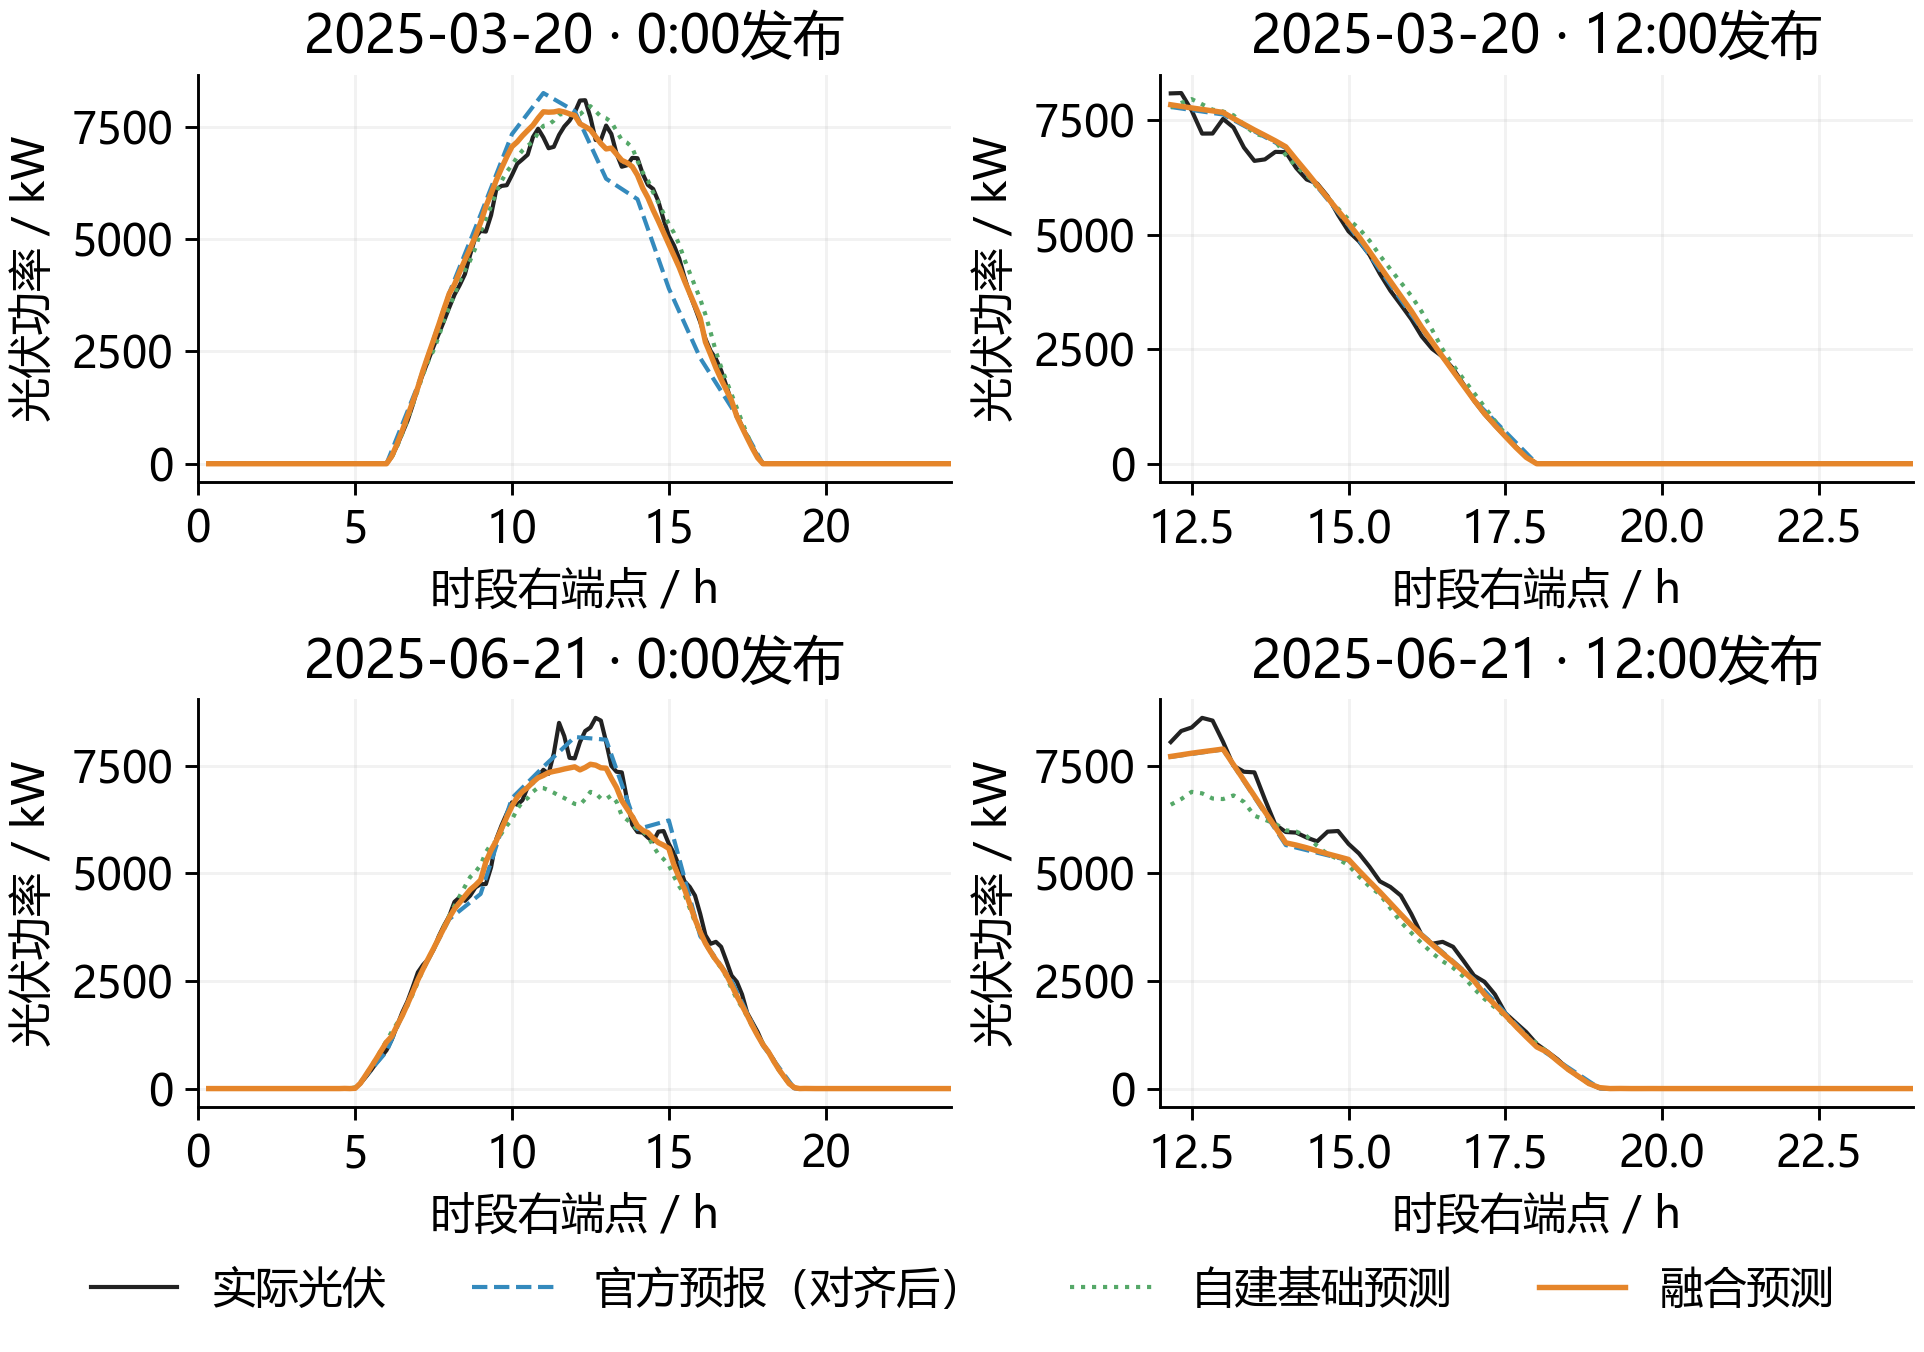
\includegraphics[width=0.90\textwidth,height=0.55\textheight,keepaspectratio]{fig11.png}
\caption*{图6 官方、自建与融合光伏预测的来源对照}
\end{figure}

记发布时刻集合为 $k\in\{0,6,12,18\}$，$k$ 表示当日零时起的发布小时数。每个发布时刻对应一个决策覆盖窗口 $J_k$（以附件 5 的计划轴 $j$ 编号）：

\begin{equation}
\begin{aligned}J_0&=\{1,\ldots,144\},&J_6&=\{36,\ldots,144\},\\ J_{12}&=\{72,\ldots,144\},&J_{18}&=\{108,\ldots,144\}.\end{aligned}
\end{equation}

这里必须区分两个时间轴。$j$ 是附件 5 定义的计划轴，$j=1$ 对应 00:10—00:20；$i$ 是自然日的物理轴，$i=1$ 对应 00:00—00:10，二者相差一个时段。0:00 发布的新计划从其覆盖窗口的第一个可自由决策时段开始，该时段在物理轴上是 $i=2$；当日 0:00—00:10 这一时段仍执行前一日计划的末尾承诺。据此，四个发布时刻对应的物理起点分别为 $i=2$、$i=37$、$i=73$、$i=109$。此前把 0:00 的物理起点记为 $i=1$ 的写法有误：它把已经由前一日计划锁定、不可再改的 00:00—00:10 时段重复计入了新计划的决策范围。

储备统计窗口与计划窗口须分别定义。$J_k$ 包含次日 00:00—00:10 段，但当天日末尚未观察到该段真实值；代码只累计当日已经完成的物理段残差。记物理残差窗口为 $I_0=\{2,\ldots,144\}$、$I_6=\{37,\ldots,144\}$、$I_{12}=\{73,\ldots,144\}$、$I_{18}=\{109,\ldots,144\}$。对发布时刻 $k$，使用该时刻自身预测版本在 $I_k$ 内的历史残差计算储备：

\begin{equation}
R_d^{(k)}=Q_{0.80}\left(\left\{\sum_{i\in I_k}\xi_{\ell,i}^{(k)}\Delta t:\ \ell<d\right\}\right)
\end{equation}

式中 $\xi_{\ell,i}^{(k)}=(L_{\ell,i}-P^{\mathrm{act}}_{\ell,i})-(L^{\mathrm{fc},(k)}_{\ell,i}-P^{\mathrm{fc},(k)}_{\ell,i})$，即实际净负荷减去相应发布时刻的模型净负荷预测；其中负荷侧为自建预测及其日内水平修正，光伏侧为官方与自建预测的融合结果。储备并非只由官方光伏预报误差估计。四个物理残差窗口分别为 143、108、72、36 段，区别于 144、109、73、37 段的计划窗口。历史样本不足 20 天时储备取零，之后按式(25)取分位数，并沿用非负截断、4800 kWh 有效上限和充电能力爬坡规则。

\subsubsection*{5.3.2 链式决策模型的建立}

按第三章假设（5），以各版承诺的路径最小值按正常电价计基准费，相邻版本之差按方向计调整费，保留该解释假设。对发布时刻 $k>0$、计划段 $j\in J_k$，记新承诺 $z=x_{d,j}^{(k)}$、上一版承诺 $p=x_{d,j}^{(k-)}$、历史最低承诺 $m=m_{d,j}^{(k-)}$，均以kW计；$(k-)$表示当前修订前的状态，而非小时数减一。下调与上调功率为 $\Delta_{d,j}^{-(k)}=[p-z]^+$、$\Delta_{d,j}^{+(k)}=[z-p]^+$；未覆盖段两者取零。按本阶段决策电价，该段费用增量为：

\begin{equation}
\Delta F_{d,j}^{(k)}=\widetilde c_{d,j}^{\mathrm{dec}}\left(\min\{m,z\}-m+0.5[p-z]^++1.5[z-p]^+\right)\Delta t
\end{equation}

第一项是基准量的变化：路径最小值只能被降低而不能被抬高，故新基准量为 $\min(m,z)$，相对原基准 $m$ 的增量如式(26)所示。第二、三项分别是向下修订的违约费与向上修订的超购费。历史最小承诺 $m$ 必不大于上一版承诺 $p$，故按新承诺 $z$ 与 $m$、$p$ 的相对位置，可把式(26)展开为三段：

\begin{equation}
\Delta F_{d,j}^{(k)}=\widetilde c_{d,j}^{\mathrm{dec}}\Delta t\begin{cases}0.5(z-m)+0.5(p-m),&0\le z<m,\\0.5(p-z),&m\le z\le p,\\1.5(z-p),&z>p.\end{cases}
\end{equation}

三段依次对应下调至历史最低承诺以下、在历史最低承诺与上一承诺之间下调、以及上调。关于 $z$ 的斜率为 $0.5\widetilde c_{d,j}^{\mathrm{dec}}\Delta t$、$-0.5\widetilde c_{d,j}^{\mathrm{dec}}\Delta t$ 与 $1.5\widetilde c_{d,j}^{\mathrm{dec}}\Delta t$，故函数连续、分段线性且非凸，不是``非线性而非分段线性''。在 $z=p$ 处值为0，在 $z=m$ 处值为 $0.5\widetilde c_{d,j}^{\mathrm{dec}}(p-m)\Delta t$。

令 $\mu=[m-z]^+$，则 $\widetilde c_{d,j}^{\mathrm{dec}}[\min\{m,z\}-m]=-\widetilde c_{d,j}^{\mathrm{dec}}\mu$。主目标与以 $\widetilde c_{d,j}^{\mathrm{dec}}\min\{m,z\}$ 作基准项的目标只差决策无关常数；代码可省略该常数。若比较求解器目标值与实际结算，还须排除终端水值和微小惩罚，并在问题四中将预测价换为实际价。最终费用按完整路径另行计算。

0:00 首次计划尚无上一版承诺和历史最低值，使用式(16)的正常购电费目标，以预测执行已锁定首段后的储电量为起点求解线性规划。6:00、12:00、18:00 修订则以当时实际储电量为起点，只覆盖各自剩余计划窗口，求解如下单阶段问题：

\begin{equation}
\min\ \sum_{j\in J_k}\Delta F_{d,j}^{(k)}-\lambda_E E_{d,T}^{\mathrm{plan},(k)}
\end{equation}

式(28)的连续决策变量为 $x_{d,j}^{(k)},u_{d,j}^{\mathrm{plan},(k)},v_{d,j}^{\mathrm{plan},(k)},w_{d,j}^{\mathrm{plan},(k)},E_{d,j}^{\mathrm{plan},(k)}$，另加结算线性化的辅助变量。输入按该发布时刻的预测重排至计划轴，末段仍采用已知首段延续值。令 $j_k=\min J_k$，修订初始状态 $E_{d,j_k-1}^{\mathrm{plan},(k)}$ 取发布时实际储电量；首次计划仍用预测锁定首段后的状态。$\lambda_E$ 取本阶段窗口电价均值乘以放电效率：

\begin{equation}
\lambda_E=\eta_d\frac{1}{|J_k|}\sum_{j\in J_k}\widetilde c_{d,j}^{\mathrm{dec}}
\end{equation}

窗口末端多留1 kWh储电可放出 $\eta_d$ kWh替代购电，故按窗口决策均价估值。各阶段单独求解，不联立优化未来发布时刻。约束沿用式(15)、(17)—(19)，将段范围替换为 $J_k$，预测、计划状态及动作增加发布时刻上标 $(k)$；储备爬坡按阶段初始状态重新计算，从 $j\ge j_k+t_{\mathrm{lo}}^{(k)}$ 起施加有效储备下界。代码仍使用式(17)后说明的微小正惩罚。

式(28)的历史最小值项非凸。引入二进制分支变量 $b^{\mathrm{bin}}$ 和辅助功率 $\mu$，在正决策电价及负系数目标下，用以下上界约束在最优解处实现 $\mu=[m-z]^+$：

\begin{equation}
\mu\le mb^{\mathrm{bin}},\qquad \mu+z+Mb^{\mathrm{bin}}\le m+M,\qquad \mu\ge0,\quad b^{\mathrm{bin}}\in\{0,1\}
\end{equation}

当 $b^{\mathrm{bin}}=1$ 时要求 $\mu+z\le m$，该分支只在 $z\le m$ 时可行；当 $b^{\mathrm{bin}}=0$ 时强制 $\mu=0$，并要求 $z\le m+M$。目标中 $\mu$ 系数为负，故在 $z<m$ 时优先选可得到 $\mu=m-z$ 的分支。约束在任意可行点不必等价于正部函数，等价性依赖最小化目标。$M$ 必须覆盖允许的承诺功率上界差，而不是无量纲常数：代码的 $10^5$ 是每段电量kWh，本文功率形式须取 $M=10^5/\Delta t=6\times10^5$ kW。本文数据下该上限远高于负荷与最大充电所需功率；它是求解分支的数值松弛，不是外网容量限制。二进制变量只用于结算分支，充放电功率仍连续。

实际结算先将各版计划映射至物理轴：$\bar x_{d,i}^{(k)}=x_{\psi(d,i)}^{(k)}$；未覆盖段沿用上一版，$i=1$ 的四版路径均来自前一计划日的尾段。记 $\bar\Delta_{d,i}^{\pm(k)}=\Delta_{\psi(d,i)}^{\pm(k)}$，其和对应相邻物理路径的方向变化。按本文结算假设，第 $d$ 天费用分为：

\begin{equation}
C_d^{\mathrm{grid}}=\sum_{i=1}^{T}c_i y_{d,i}^{\mathrm{base}}\Delta t,\qquad y_{d,i}^{\mathrm{base}}=\min_{k\in\mathcal K}\bar x_{d,i}^{(k)}
\end{equation}

\begin{equation}
C_d^{\mathrm{adj}}=\sum_{i=1}^{T}c_i\left(0.5\sum_{k\in\mathcal K\setminus\{0\}}\bar\Delta_{d,i}^{-(k)}+1.5\sum_{k\in\mathcal K\setminus\{0\}}\bar\Delta_{d,i}^{+(k)}\right)\Delta t
\end{equation}

\begin{equation}
C_d^{\mathrm{emer}}=\sum_{i=1}^{T}5c_i e_{d,i}\Delta t
\end{equation}

三式之和为 $C_d=C_d^{\mathrm{grid}}+C_d^{\mathrm{adj}}+C_d^{\mathrm{emer}}$。其中 $y_{d,i}^{\mathrm{base}}$ 是路径最小结算功率，不是实际使用功率 $y_{d,i}$，也不是最终生效承诺 $x_{d,i}^{\mathrm{exec}}$。问题四的实际结算将固定电价 $c_i$ 替换为实际电价 $c_{d,i}$。

求解得到窗口内各时段的承诺量后，进入执行层。执行层不接收储备量 $R$，也不求解任何优化问题，只把该时段最终生效的承诺量 $x_{d,i}^{\mathrm{exec}}$ 与实际负荷、实际光伏一起作为已知输入，按"无未来信息可得"的现实条件逐时段推进。为统一描述充放电的触发条件，先定义该时段的\textbf{供需余量} $s_{d,i}=x_{d,i}^{\mathrm{exec}}+P_{d,i}^{\mathrm{act}}-L_{d,i}$：$s_{d,i}\ge0$ 表示供大于需，$s_{d,i}<0$ 表示需大于供。充放电规则按 $s_{d,i}$ 的符号分为两支，两式中的取小项同时计入功率上限与储电量边界，保证执行过程不越界：

\begin{equation}
s_{d,i}\ge0:\quad u_{d,i}=\min\left(s_{d,i},\ P_{st}^{\max},\ \frac{E_{\max}-E_{d,i-1}^{\mathrm{act}}}{\eta_c\Delta t}\right),\qquad v_{d,i}=0
\end{equation}

\begin{equation}
s_{d,i}<0:\quad v_{d,i}=\min\left(-s_{d,i},\ P_{st}^{\max},\ \frac{\eta_d\left(E_{d,i-1}^{\mathrm{act}}-E_{\min}\right)}{\Delta t}\right),\qquad u_{d,i}=0
\end{equation}

两式之外的动作不参与优化，只按式(20)的实际功率平衡逐项清算，依次为：光伏实际出力先供负载与充电，即 $g_{d,i}=\min\{P_{d,i}^{\mathrm{act}},\,L_{d,i}+u_{d,i}\}$，余下部分弃光，$w_{d,i}=P_{d,i}^{\mathrm{act}}-g_{d,i}$；承诺量中真正被使用的部分为 $y_{d,i}=\min\{x_{d,i}^{\mathrm{exec}},\,[L_{d,i}+u_{d,i}-g_{d,i}]^{+}\}$，与承诺量之差 $r_{d,i}=x_{d,i}^{\mathrm{exec}}-y_{d,i}$ 即\textbf{已承诺但未使用的功率}，对应每段未用电量为 $r_{d,i}\Delta t$；放电用满（$v_{d,i}$ 取到取小项中的某一项）仍不足以补足缺口时，差额 $e_{d,i}=[-s_{d,i}-v_{d,i}]^{+}$ 转为紧急购电，按同时段电价的 5 倍计入当日结算。执行层每一步都是逐个时段的局部判断，不使用任何未来时段的信息。

\subsubsection*{5.3.3 问题三模型的求解}

问题三的求解分两层。计划层在四个发布时刻各求解一次单阶段问题：0:00 为线性规划，6:00、12:00、18:00 为含 0-1 变量的混合整数线性规划，由 HiGHS 的分支定界与割平面求解，每个单阶段的变量与约束条数都随时段数线性增长，与年份长度无关。执行层不求解优化问题，只按式(34)、(35)逐时段贪心推进，因此执行层不会引入额外的求解规模，也不会出现"执行层不可解"的情况。

与问题二相比，问题三的计算量约增加一倍：每日由 1 次计划变为 4 次，其中 3 次为混合整数问题。正式评价期 334 天的全年回放耗时约 89 秒，折算单日约 0.27 秒，仍然远短于 10 分钟的控制间隔。求解器参数与问题二完全一致：HiGHS 默认分支定界、梯度提升树固定随机种子并单线程运行。为保证四个子问题可比，全部实验使用同一套代码与同一份冻结数据，未针对任一子问题单独调参。

\subsubsection*{5.3.4 问题三结果的分析}

正式评价期 334 天，问题三总费用 13,439,044.37 元，比问题二低 425,594.99 元（42.56 万元），降幅 3.07\%。费用构成为：基准费 12,420,152.72 元（占 92.42\%）、下调费 176,679.68 元（1.31\%）、上调费 715,045.71 元（5.32\%）、紧急购电费 127,166.25 元（0.95\%）。全年首次计划购电量 20,374,636.63 kWh，最终有效承诺购电量 20,618,426.53 kWh，两者相差 243,789.90 kWh，即 6:00、12:00、18:00 三次修订在净额上把承诺量向上抬了约 1.20\%；全年调整电量合计 1,288,029.77 kWh，占首次计划量的 6.32\%。上调与下调的费用之比为 4.05，电量之比为 1.47，可见调整的方向与量级并不对称。

问题三的完整结果见表 8，其结构与表 7 一致，便于逐项对照。需要强调的是，表 8 中六个指定时段的购电量与"全天最终有效承诺购电量"给出的是\textbf{当日 18:00 修订后的最终承诺量}，而"全天首次计划购电量"是 0:00 的首次计划量；两者含义不同，不能混用。

{\fontsize{9.5}{11.5}\selectfont
\begin{longtable}{C{\dimexpr0.360000\textwidth-2\tabcolsep\relax}C{\dimexpr0.160000\textwidth-2\tabcolsep\relax}C{\dimexpr0.160000\textwidth-2\tabcolsep\relax}C{\dimexpr0.160000\textwidth-2\tabcolsep\relax}C{\dimexpr0.160000\textwidth-2\tabcolsep\relax}}
\caption*{表8 问题三在指定时间段的购电量、全天购电费及紧急购电情况（正式评价期）}\\
\toprule
\textbf{项目} & \textbf{2025-03-20} & \textbf{2025-06-21} & \textbf{2025-09-23} & \textbf{2025-12-21} \\
\midrule
\endfirsthead
\toprule
\textbf{项目} & \textbf{2025-03-20} & \textbf{2025-06-21} & \textbf{2025-09-23} & \textbf{2025-12-21} \\
\midrule
\endhead
时段 10:00-10:10 购电量 / kWh & 0.00 & 0.00 & 0.00 & 68.97 \\
时段 12:00-12:10 购电量 / kWh & 537.72 & 0.00 & 367.69 & 909.20 \\
时段 14:00-14:10 购电量 / kWh & 0.00 & 0.00 & 0.00 & 0.00 \\
时段 16:00-16:10 购电量 / kWh & 489.92 & 149.66 & 564.78 & 826.02 \\
时段 18:00-18:10 购电量 / kWh & 707.76 & 422.11 & 774.77 & 707.86 \\
时段 20:00-20:10 购电量 / kWh & 0.00 & 0.00 & 0.00 & 0.00 \\
全天首次计划购电量 / kWh & 65,209.37 & 36,250.37 & 66,931.47 & 92,272.34 \\
全天最终有效承诺购电量 / kWh & 66,572.53 & 36,189.35 & 66,620.99 & 94,103.71 \\
全天购电费 / 元 & 44,976.91 & 21,389.62 & 43,704.61 & 62,855.00 \\
当天紧急购电量 / kWh & 0.00 & 0.00 & 6.38 & 54.93 \\
当天紧急购电费 / 元 & 0.00 & 0.00 & 43.00 & 319.70 \\
0:00 储电量 / kWh & 10,370.85 & 10,306.88 & 9,693.46 & 9,608.44 \\
24:00 储电量 / kWh & 10,152.97 & 10,556.60 & 9,741.32 & 9,843.16 \\
00:00—04:00 充电量 / kWh & 583.81 & 615.65 & 1,196.39 & 1,071.65 \\
00:00—04:00 放电量 / kWh & 351.88 & 3,025.35 & 110.95 & 299.02 \\
04:00—08:00 充电量 / kWh & 96.04 & 346.22 & 251.89 & 1,553.61 \\
04:00—08:00 放电量 / kWh & 4,995.21 & 4,824.66 & 5,519.66 & 1,634.80 \\
08:00—12:00 充电量 / kWh & 2,738.57 & 9,277.40 & 3,408.10 & 4,317.25 \\
08:00—12:00 放电量 / kWh & 2,777.38 & 0.00 & 1,896.62 & 6,686.80 \\
12:00—16:00 充电量 / kWh & 6,426.62 & 0.00 & 5,821.75 & 7,298.74 \\
12:00—16:00 放电量 / kWh & 378.69 & 0.00 & 505.36 & 2,592.11 \\
16:00—20:00 充电量 / kWh & 201.25 & 0.00 & 111.25 & 80.35 \\
16:00—20:00 放电量 / kWh & 5,273.79 & 4,755.36 & 4,864.44 & 5,396.32 \\
20:00—24:00 充电量 / kWh & 9,485.28 & 8,732.77 & 8,510.60 & 9,135.71 \\
20:00—24:00 放电量 / kWh & 2,239.72 & 2,537.25 & 2,692.89 & 2,180.13 \\
全天充电量 / kWh & 19,531.58 & 18,972.04 & 19,299.98 & 23,457.31 \\
全天放电量 / kWh & 16,016.67 & 15,142.61 & 15,589.91 & 18,789.17 \\
\bottomrule
\end{longtable}
{\footnotesize\par\vspace{2pt}注：六个指定时段的购电量与「全天最终有效承诺购电量」为当日 18:00 修订后的最终承诺量；「全天首次计划购电量」为 00:00 首次计划量。全天购电费按题面结算口径给出，基准费以路径最小承诺结算基准量计价，另叠加下调费、上调费与紧急购电费，故不等于任一承诺量乘以电价。\par}
}

\begin{figure}[H]
\centering

\includegraphics[width=0.90\textwidth,height=0.55\textheight,keepaspectratio]{fig06.png}
\caption*{图7 问题三某一日承诺路径的分阶段修订阶梯}
\end{figure}

\begin{figure}[H]
\centering

\includegraphics[width=0.90\textwidth,height=0.55\textheight,keepaspectratio]{fig07.png}
\caption*{图8 问题三四个指定日期的调度曲线}
\end{figure}

\begin{figure}[H]
\centering

\includegraphics[width=0.90\textwidth,height=0.55\textheight,keepaspectratio]{fig08.png}
\caption*{图9 问题三逐日费用构成}
\end{figure}

图7 以 2025-07-01 为例展示承诺路径的阶梯形态：0:00 的首次计划给出全天基础轮廓，6:00 与 12:00 的修订主要发生在光伏出力不确定的白天，18:00 的修订幅度最小。图8 给出四个指定日期的储电量、购电量与光伏曲线，形态与表 8 的数值一致。图9 的逐日费用构成说明四类费用中基准费占绝对主导，调整费与紧急费只在少数日期出现明显尖峰。

与问题二的对比还须注意一点：问题三比问题二少花 42.56 万元，这是\textbf{整个系统在两种发布机制、不同预测配置、两套储备统计与两种执行方式共同作用下的净收益}，不能全部归因于"多次调整"这一项。问题三同时改变了预测层的融合方式、储备层的统计窗口与执行层的推进方式，三者对结果的贡献相互交织；本文不做逐项因果分解，"多次调整"的独立价值只能通过 5.3.5 节的消融实验在同一配置内部观察。

\subsubsection*{5.3.5 发布时点的价值与消融实验}

为考察各日内发布时点的价值，本文固定其余设置，只改变启用时点的组合，在正式评价期 334 天上回放。启用某时点意味着同时接入该时刻的官方光伏预报及对应融合结果、更新自建负荷预测的剩余段水平、使用该时点的储备统计并重新决策。因此，这项消融测量的是该时点预测更新与重新决策的综合价值，不能解释为官方光伏预报单独的经济价值，也不能解释为只增加一次求解的独立收益。结果见表9，全部数据来自同一套代码的同一次批量实验，未重新调参。

\begin{table}[H]
\centering\fontsize{9.5}{11.5}\selectfont
\caption*{表9 发布时点消融：正式评价期 334 天各时点启用组合与总费用}
\begin{tabular}{C{\dimexpr0.360000\textwidth-2\tabcolsep\relax}C{\dimexpr0.160000\textwidth-2\tabcolsep\relax}C{\dimexpr0.160000\textwidth-2\tabcolsep\relax}C{\dimexpr0.160000\textwidth-2\tabcolsep\relax}C{\dimexpr0.160000\textwidth-2\tabcolsep\relax}}
\toprule
\textbf{启用时点} & \textbf{问题三费用 / 元} & \textbf{问题三相对完整配置} & \textbf{问题 4-3 费用 / 元} & \textbf{问题 4-3 相对完整配置} \\
\midrule
仅 0:00 & 13,893,004.63 & +453,960 元 & 14,630,594.80 & +472,469 元 \\
0:00 + 6:00 & 13,614,459.44 & +175,415 元 & 14,330,087.45 & +171,962 元 \\
0:00 + 12:00 & 13,449,334.14 & +10,290 元 & 14,164,446.47 & +6,321 元 \\
0:00 + 18:00 & 13,460,892.18 & +21,848 元 & 14,183,662.90 & +25,537 元 \\
0:00 + 6:00 + 12:00（关闭 18:00） & 13,502,211.17 & +63,167 元 & 14,200,388.31 & +42,263 元 \\
0:00 + 12:00 + 18:00（关闭 6:00） & 13,371,325.06 & -67,719 元 & 14,098,901.92 & -59,224 元 \\
0:00 + 6:00 + 18:00（关闭 12:00） & 13,463,094.72 & +24,050 元 & 14,182,371.25 & +24,246 元 \\
0:00 + 6:00 + 12:00 + 18:00（完整配置） & 13,439,044.37 & — & 14,158,125.73 & — \\
\bottomrule
\end{tabular}
{\footnotesize\par\vspace{2pt}注：相对完整配置 = 该组合费用 − 完整配置费用，负值表示比完整配置更省。表中全部组合均由同一套代码在正式评价期 334 天上回放得到，未重新调参。\par}
\end{table}

表中数值给出两个层次的信息，必须分开读。

第一层是\textbf{单点启用价值}：以"仅 0:00"为参照，单独增加一个发布时点所能节省的费用。问题三中单独增加 6:00 节省 27.85 万元，单独增加 12:00 节省 44.37 万元，单独增加 18:00 节省 43.21 万元；问题 4-3 中三个数值分别为 30.05 万元、46.61 万元与 44.69 万元。三个时点的单点价值都很大且量级相近。

第二层是\textbf{完整配置下的边际价值}：在四个时点全部启用的基础上，关掉某一个时点会使费用增加多少。问题三中关掉 12:00 多花 24,050.35 元，关掉 18:00 多花 63,166.80 元，而关掉 6:00 反而\textbf{少花} 67,719.31 元；问题 4-3 中对应数值为多花 24,245.51 元、多花 42,262.58 元与少花 59,223.82 元。

单点启用价值与完整配置下边际价值的差距，说明时点之间存在明显交互：6:00 单独启用时节省 27.85 万元，但在 12:00 与 18:00 都启用时，它的边际价值为负。后续时点会用新官方光伏预报的融合结果和已观测负荷修正更新剩余计划，较早的承诺修订还会影响后续调整费与储能状态；这些因素可能共同导致额外时点不再降低费用。消融结果本身不能证明后续官方预报完全包含较早预报的信息，也不能确定负边际价值只由预报重叠造成。因此本文的结论限定为：\textbf{正式评价期 334 天内，在本文既定预测、储备与执行配置下，关闭 6:00 比保留更经济；12:00 与 18:00 在完整配置下具有正边际价值。}

这一结论不能外推到自然年口径。在自然年 365 天的口径下，问题 4-3 关闭 6:00 会使费用从 16,218,310.91 元上升到 16,228,758.96 元，\textbf{反而多花 10,448.05 元}。正式期与自然年的差别在于是否包含 1 月：1 月是预跑期，储电量在这一个月内由初始值演化到 2 月 1 日的水平，6:00 的提前修订在预跑期改变了储电量的演化路径，进而影响到正式期起点的储电量状态。同一项消融在两个口径下符号相反，说明"关闭 6:00"的收益依赖评价期的选取，本文不把它作为普遍建议。

本文正式交付的方案仍是四个时点全部启用的完整配置（表9 中的「完整配置」）。关闭 6:00 是在同一配置内部观察到的一次消融改进，其收益（6.77 万元）只占完整配置总费用的 0.50\%，且仅在正式期口径下成立，故本文报告该现象但不替换正式基线：一方面替换基线会使表 8、表9 中已冻结的正式结果全部失效，另一方面单一口径下的 0.50\% 改进不足以支撑"应当关闭"的一般性结论。这一点也说明了本文策略的时点启用配置仍有优化空间，属于 7.2 节列出的改进方向之一。

\needspace{3\baselineskip}\subsection*{5.4 问题四模型的建立与求解}

\subsubsection*{5.4.1 实时电价的预测}

问题四把附件 1 的固定电价替换为附件 4 的实时电价，其余条件不变，因此需要在问题二、问题三的模型上增加一个电价预测通道。本文按与负荷、光伏相同的方式处理电价：只用预测时点之前已经发生的历史电价建模，对当日 144 个时段逐点预测，预测在当日 0:00 一次性生成，日内不再更新。问题 4-2 与问题 4-3 分别沿用问题二与问题三的决策与执行结构，只是把其中的电价替换为预测电价。

附件 4 的实时电价有两个统计特征需要在建模时考虑。第一，它的全年均值为 0.766198 元/kWh，与附件 1 的固定电价均值 0.766197 元/kWh 几乎完全相等，但日内波动显著：逐时段的标准差平均为 0.1238 元/kWh、最大为 0.2234 元/kWh，相当于年均价的 16.2\%—29.2\%；日均价的年内变化区间为 0.5378—0.9290 元/kWh，最高日与最低日之比为 1.727。第二，价格波动的时间尺度以日为主，日内形态在不同日期之间并不稳定。

均值的相等与波动的存在这两件事放在一起，恰好说明问题四的费用变化不可能来自电价水平——但\textbf{也不能反过来说费用差与电价无关}。总购电费是购电量与购电时点电价的乘积之和，是一个按购电量加权的购电时点价格。全年均价相同只意味着简单平均相同，若某策略把购电集中到低价时段，其加权均价会低于 0.766198，费用随之下降。因此问题 4-2、4-3 与问题二、问题三的费用差既包含购电量的差异，也包含购电时点结构的差异，本文按后者单独统计加权均价来说明这一点，不把费用差简单归因于任何单一来源。

\subsubsection*{5.4.2 决策与结算的分离}

问题四的模型结构在三个层面上把"预测"、"决策"与"结算"分开，这是与前三问最值得说明的建模选择。

第一层是\textbf{决策用预测价、结算用实际价}。优化模型中的目标函数使用当日 0:00 生成的预测电价序列 $\widetilde c_{d,j}^{\mathrm{dec}}$，据此决定各时段的购电量与充放电计划；而全天费用的结算使用附件 4 给出的实际电价 $c_{d,i}$。两者不混用：把实际电价代入决策目标等价于使用了当日 0:00 尚不可得的信息，属于前视偏差，会人为压低费用、使结果不可实施。

第二层是\textbf{电价预测在日内不更新，负荷与光伏预测按信息条件更新}。这一处理与题目条件一致：附件 3 只提供光伏的发布时点预测，没有提供电价的发布时点预测。因此在问题 4-3 中，三个发布时点会带来更新的负荷与光伏预测，但电价预测始终是 0:00 的那一版。这一点使问题 4-3 与问题三在信息结构上并不完全平行，也是问题 4-3 相对问题三费用增加的主要原因之一。

第三层是\textbf{结算口径与前三问保持一致}。问题 4-2 沿用问题二的"全天单一承诺量"口径，问题 4-3 沿用问题三的"路径最小承诺量 + 逐次调整费"口径，均不做修改。本文对多版承诺的合成方式采用项目自定的解释口径（见 第三章假设（6））：题面只规定了基准量与调整费的方向性费率，没有给出官方解释文件，因此本文按项目声明的口径实现并在全文中保持同一口径，四个子问题的费用数字因此可比。

除外，问题 4-2 与问题 4-3 的目标函数、功率平衡、储电量约束与执行层结构与问题二、问题三完全相同，此处不再重复列出，只补充两个子问题的总费用合成式。

两个子问题的总费用按上述口径合成。问题 4-2 只有一次计划承诺，其费用为

\begin{equation}
C_{4\text{-}2}=\sum_{d=32}^{D}\sum_{i=1}^{T}c_{d,i}\left(x_{d,i}^{\mathrm{exec}}+5e_{d,i}\right)\Delta t
\end{equation}

问题 4-3 在同样口径上叠加逐次调整费：

\begin{equation}
\begin{aligned}C_{4\text{-}3}=\sum_{d=32}^{D}\sum_{i=1}^{T}c_{d,i}\Delta t\Bigg[&y_{d,i}^{\mathrm{base}}+5e_{d,i}\\ &+0.5\sum_{k\in\mathcal K\setminus\{0\}}\bar\Delta_{d,i}^{-(k)}+1.5\sum_{k\in\mathcal K\setminus\{0\}}\bar\Delta_{d,i}^{+(k)}\Bigg].\end{aligned}
\end{equation}

两式中的电价一律取附件 4 的实际电价 $c_{d,i}$，即"决策用预测价、结算用实际价"中的结算侧。

\subsubsection*{5.4.3 问题四结果的分析}

正式评价期 334 天，问题 4-2 总费用 14,595,194.94 元，问题 4-3 总费用 14,158,125.73 元；问题 4-3 比问题 4-2 低 437,069.21 元（43.71 万元），降幅 2.99\%。与问题二、问题三相比，两个子问题的费用分别高出 730,555.58 元与 719,081.36 元。

这一价差需要谨慎解读。附件 4 与附件 1 的全年均价几乎相同，因此价差不可能来自电价的\textbf{平均水平}；但"均价相同"只约束简单平均，不约束电价的时间结构——附件 4 的逐日、逐时段电价与附件 1 的固定曲线在形态上完全不同。因此这 73.06 万元中至少混合了三个来源：一是实际电价时间结构本身的变化带来的购电成本变化；二是电价预测误差使部分购电落在并非最低价的时段，抬高按购电量加权的购电均价；三是电价波动扩大了决策的风险面，同样的储备水平在波动电价下的期望费用更高。本文只报告加权均价的差异，不对这三个来源做定量分离，也不把价差单独归因于电价预测误差。若要单独度量电价预测误差的价值，只能看 6.2 节表 11 中 C2 与 C3 的差额（问题 4-2 为 7.68 万元、问题 4-3 为 7.75 万元），该差额才是在其余条件完全相同、仅电价信息不同时测得的。

问题 4-2 与 4-3 的完整结果见表10，两个子问题并排给出，便于与表 7、表 8 对照。

{\fontsize{9.5}{11.5}\selectfont
\begin{longtable}{C{\dimexpr0.360000\textwidth-2\tabcolsep\relax}C{\dimexpr0.160000\textwidth-2\tabcolsep\relax}C{\dimexpr0.160000\textwidth-2\tabcolsep\relax}C{\dimexpr0.160000\textwidth-2\tabcolsep\relax}C{\dimexpr0.160000\textwidth-2\tabcolsep\relax}}
\caption*{表10(a) 问题 4-2 与 4-3 在指定时间段的购电量、全天购电费及紧急购电情况（正式评价期）}\\
\toprule
\textbf{项目} & \textbf{4-2 03-20} & \textbf{4-2 06-21} & \textbf{4-2 09-23} & \textbf{4-2 12-21} \\
\midrule
\endfirsthead
\toprule
\textbf{项目} & \textbf{4-2 03-20} & \textbf{4-2 06-21} & \textbf{4-2 09-23} & \textbf{4-2 12-21} \\
\midrule
\endhead
时段 10:00-10:10 购电量 / kWh & 0.00 & 0.00 & 0.00 & 0.00 \\
时段 12:00-12:10 购电量 / kWh & 544.56 & 0.00 & 0.00 & 906.64 \\
时段 14:00-14:10 购电量 / kWh & 0.00 & 0.00 & 0.00 & 0.00 \\
时段 16:00-16:10 购电量 / kWh & 466.12 & 181.46 & 542.57 & 800.85 \\
时段 18:00-18:10 购电量 / kWh & 701.84 & 457.02 & 0.00 & 711.50 \\
时段 20:00-20:10 购电量 / kWh & 736.00 & 0.00 & 148.83 & 0.00 \\
全天首次计划购电量 / kWh & 64,856.44 & 36,839.27 & 66,212.60 & 92,218.98 \\
全天最终有效承诺购电量 / kWh & 64,856.44 & 36,839.27 & 66,212.60 & 92,218.98 \\
全天购电费 / 元 & 43,048.85 & 19,450.56 & 46,003.46 & 71,720.50 \\
当天紧急购电量 / kWh & 257.52 & 0.00 & 11.32 & 32.08 \\
当天紧急购电费 / 元 & 1,207.73 & 0.00 & 73.78 & 226.29 \\
0:00 储电量 / kWh & 9,880.45 & 10,302.49 & 9,835.15 & 9,648.76 \\
24:00 储电量 / kWh & 8,835.02 & 10,580.82 & 9,685.14 & 8,629.20 \\
00:00—04:00 充电量 / kWh & 1,180.07 & 703.90 & 688.13 & 1,436.97 \\
00:00—04:00 放电量 / kWh & 318.85 & 6,104.68 & 90.71 & 308.25 \\
04:00—08:00 充电量 / kWh & 971.79 & 1,178.56 & 1,410.78 & 267.13 \\
04:00—08:00 放电量 / kWh & 5,089.83 & 1,812.69 & 5,124.46 & 980.78 \\
08:00—12:00 充电量 / kWh & 3,108.22 & 8,444.86 & 2,583.64 & 4,243.42 \\
08:00—12:00 放电量 / kWh & 2,777.38 & 0.00 & 1,896.62 & 6,232.40 \\
12:00—16:00 充电量 / kWh & 4,484.65 & 0.00 & 5,005.96 & 6,651.55 \\
12:00—16:00 放电量 / kWh & 653.17 & 0.00 & 589.00 & 2,694.21 \\
16:00—20:00 充电量 / kWh & 130.07 & 20.35 & 140.56 & 51.95 \\
16:00—20:00 放电量 / kWh & 5,878.76 & 4,055.37 & 4,251.83 & 3,988.58 \\
20:00—24:00 充电量 / kWh & 8,445.23 & 7,866.90 & 7,868.27 & 7,326.78 \\
20:00—24:00 放电量 / kWh & 1,062.11 & 2,530.57 & 2,517.23 & 2,895.39 \\
全天充电量 / kWh & 18,320.02 & 18,214.57 & 17,697.34 & 19,977.79 \\
全天放电量 / kWh & 15,780.10 & 14,503.31 & 14,469.85 & 17,099.61 \\
\bottomrule
\end{longtable}
{\footnotesize\par\vspace{2pt}注：购电量均为最终有效承诺量。全天购电费按题面结算口径给出，含基准费、调整费与紧急购电费；4-2 当天仅一次计划，最终有效承诺量等于首次计划量。\par}
}

{\fontsize{9.5}{11.5}\selectfont
\begin{longtable}{C{\dimexpr0.360000\textwidth-2\tabcolsep\relax}C{\dimexpr0.160000\textwidth-2\tabcolsep\relax}C{\dimexpr0.160000\textwidth-2\tabcolsep\relax}C{\dimexpr0.160000\textwidth-2\tabcolsep\relax}C{\dimexpr0.160000\textwidth-2\tabcolsep\relax}}
\caption*{表10(b) 问题 4-2 与 4-3 在指定时间段的购电量、全天购电费及紧急购电情况（正式评价期）}\\
\toprule
\textbf{项目} & \textbf{4-3 03-20} & \textbf{4-3 06-21} & \textbf{4-3 09-23} & \textbf{4-3 12-21} \\
\midrule
\endfirsthead
\toprule
\textbf{项目} & \textbf{4-3 03-20} & \textbf{4-3 06-21} & \textbf{4-3 09-23} & \textbf{4-3 12-21} \\
\midrule
\endhead
时段 10:00-10:10 购电量 / kWh & 0.00 & 0.00 & 0.00 & 0.00 \\
时段 12:00-12:10 购电量 / kWh & 537.72 & 0.00 & 369.11 & 909.20 \\
时段 14:00-14:10 购电量 / kWh & 0.00 & 0.00 & 0.00 & 0.00 \\
时段 16:00-16:10 购电量 / kWh & 530.81 & 149.66 & 564.78 & 826.02 \\
时段 18:00-18:10 购电量 / kWh & 707.76 & 455.58 & 0.00 & 707.86 \\
时段 20:00-20:10 购电量 / kWh & 743.21 & 0.00 & 0.00 & 0.00 \\
全天首次计划购电量 / kWh & 65,209.37 & 36,408.70 & 67,277.42 & 92,112.62 \\
全天最终有效承诺购电量 / kWh & 66,699.71 & 36,278.67 & 67,302.60 & 93,977.21 \\
全天购电费 / 元 & 45,798.44 & 18,739.21 & 46,116.13 & 73,367.17 \\
当天紧急购电量 / kWh & 0.00 & 0.00 & 11.32 & 54.93 \\
当天紧急购电费 / 元 & 0.00 & 0.00 & 73.78 & 390.04 \\
0:00 储电量 / kWh & 10,439.72 & 10,321.92 & 9,751.83 & 9,609.69 \\
24:00 储电量 / kWh & 10,153.79 & 10,649.68 & 10,331.72 & 9,851.58 \\
00:00—04:00 充电量 / kWh & 507.29 & 686.58 & 1,084.92 & 1,466.52 \\
00:00—04:00 放电量 / kWh & 351.88 & 6,696.76 & 110.95 & 283.91 \\
04:00—08:00 充电量 / kWh & 914.04 & 1,177.79 & 298.51 & 267.22 \\
04:00—08:00 放电量 / kWh & 5,654.88 & 1,830.16 & 5,519.66 & 963.12 \\
08:00—12:00 充电量 / kWh & 2,738.57 & 9,193.88 & 3,408.10 & 4,231.16 \\
08:00—12:00 放电量 / kWh & 2,777.38 & 0.00 & 1,896.62 & 6,735.84 \\
12:00—16:00 充电量 / kWh & 6,389.79 & 0.00 & 5,801.25 & 7,369.77 \\
12:00—16:00 放电量 / kWh & 378.69 & 0.00 & 483.72 & 2,532.04 \\
16:00—20:00 充电量 / kWh & 186.12 & 20.24 & 100.45 & 89.33 \\
16:00—20:00 放电量 / kWh & 5,993.61 & 4,616.24 & 4,848.74 & 4,652.31 \\
20:00—24:00 充电量 / kWh & 9,465.40 & 8,631.32 & 9,146.33 & 9,145.30 \\
20:00—24:00 放电量 / kWh & 1,463.90 & 2,526.81 & 2,688.45 & 2,896.23 \\
全天充电量 / kWh & 20,201.21 & 19,709.82 & 19,839.56 & 22,569.31 \\
全天放电量 / kWh & 16,620.33 & 15,669.97 & 15,548.14 & 18,063.44 \\
\bottomrule
\end{longtable}
{\footnotesize\par\vspace{2pt}注：购电量均为最终有效承诺量。全天购电费按题面结算口径给出，含基准费、调整费与紧急购电费；4-2 当天仅一次计划，最终有效承诺量等于首次计划量。\par}
}

\begin{figure}[H]
\centering

\includegraphics[width=0.90\textwidth,height=0.55\textheight,keepaspectratio]{fig09.png}
\caption*{图10 四个指定日期与全年平均的实时电价曲线}
\end{figure}

\begin{figure}[H]
\centering

\includegraphics[width=0.90\textwidth,height=0.55\textheight,keepaspectratio]{fig10.png}
\caption*{图11 问题 4-2 与问题 4-3 的指标对比}
\end{figure}

图10 给出四个指定日期的实时电价曲线与全年均价线。四个日期的日内形态差异明显，且各日的均值线并不都落在全年均价线上，说明"全年均价相同"掩盖了显著的日内与日内间差异；这也正是 5.4.1 节强调不能用全年均价相等来推断费用差与电价无关的原因。图11 从总购电费用、日费用标准差、总购电量与调整电量四个维度对比 4-2 与 4-3。需要说明的是，计划调整是问题 4-3 独有的机制，问题 4-2 只发布一次全天承诺、不存在调整量，因此调整电量一栏只有 4-3 有定义，不与 4-2 作比较；两个子问题可比的是总费用与总购电量，4-3 在这两项上均低于 4-2。

需要提醒的是，问题 4-3 中 6:00、12:00、18:00 三个时点带来的负荷与光伏信息更新确实降低了购电需求，但电价预测在日内不更新，因此三个时点的修订只能在电力侧而非价格侧发挥作用。这与问题三的情况不同：问题三的四个时点在信息结构上是完整的，问题 4-3 则只有一半。两者费用降幅接近（3.07\% 与 2.99\%）说明在本文数据下，时点信息的主要价值来自负荷与光伏侧而非价格侧。

\subsubsection*{5.4.4 电价波动下的策略比较}

把四个子问题的结果放在一起，可以给出三条在本文数据范围内成立的结论。

第一，\textbf{费用对实时电价的时间结构是敏感的}。问题 4-2 与问题二使用完全相同的决策结构与执行结构，唯一区别是电价由固定价换成实时价的预测值，费用上升 730,555.58 元。这一价差不含电价平均水平的变化（两者年均价相同），但如 5.4.3 节所述，它同时混有实际电价时间结构与预测误差两方面的作用，本文不把它单独归因于电价预测误差。

第二，\textbf{多次修订在电价波动下依然有效}。问题 4-3 相对问题 4-2 节省 43.71 万元，与问题三相对问题二节省的 42.56 万元量级一致，说明链式修订的收益并不依赖于电价是否固定。

第三，\textbf{储备水平在四个（子）问题中都是费用的主要控制变量，但"电价波动使储备作用更强"这一说法在本文数据下只有很弱的证据}。以各自的 $q=0.80$ 结果为基准（问题二 13,864,639.36 元、问题三 13,439,044.37 元、问题 4-2 14,595,194.94 元、问题 4-3 14,158,125.73 元），表 12 中 $q$ 下调到 0.50 时费用分别升至 14,854,881.11 元、13,533,398.79 元、15,641,955.75 元与 14,280,014.41 元，绝对增幅为 99.02 万元、9.44 万元、104.68 万元与 12.19 万元，相对增幅为 7.14\%、0.70\%、7.17\% 与 0.86\%。逐对比较可见：问题 4-2 的绝对与相对增幅都略大于问题二，问题 4-3 也略大于问题三，方向一致；但问题二与问题 4-2 的相对增幅几乎相同（7.14\% 与 7.17\%），问题三与问题 4-3 的差距也主要来自基数不同。因此本文只报告"四个（子）问题的费用都对储备水平高度敏感、储备层不是可有可无的装饰"，不主张电价波动显著放大了储备的价值。上述数值仅反映当前配置下的参数敏感性。储备量不直接进入执行器，而是通过计划承诺间接影响运行；不同问题还采用不同预测配置和执行方式，因此本文不将费用增幅差异归因于某一种执行机制。

最后需要说明本文结果不支持的表述。全年紧急购电费占总费用的比例不足 1\%（问题三为 0.95\%，问题 4-3 为 0.92\%），但\textbf{不能由此得出"事后补缺口比事前储备便宜"的结论}：紧急购电的价格是同时段正常电价的 5 倍，它占比低只是因为本文储备设置把缺口压得很小，一旦储备水平下调，紧急购电量与费用都会迅速上升（见表 12，$q=0.50$ 时问题三紧急购电量由 21,542 kWh 升至 102,007 kWh）。占比低恰恰是储备有效的结果，而不是可以放松储备的理由。

\needspace{4\baselineskip}\section*{六、模型检验}

\needspace{3\baselineskip}\subsection*{6.1 物理可行性与数值精度的核验}

本文对四个子问题的全年逐时段结果都做了物理可行性核验，核验对象为 52,560 个物理时段（365 天 $\times$ 144 时段）的全量记录，核验项与结果如下。

功率平衡残差：以"购电 + 光伏实际可用 + 放电 = 负荷 + 充电"与"光伏实际可用 + 弃光 = 光伏出力"两式逐时段核验，四个子问题的折算为每段电量后的最大残差均为 $2.27\times10^{-13}$ kWh，属于双精度浮点的舍入量级，不构成物理失衡。摘要所引的即为此值。

边界与逻辑约束：储电量越界时段数 0 个，充放电功率越界时段数 0 个，同时充放电时段数 0 个，反向购电（购电量为负）时段数 0 个。四个子问题的年末储电量均为 6000.0 kWh，达到本文设定的年末收口目标（见 第三章假设（6））；题面只规定了 2025 年 1 月 1 日 0:00 的初始储电量为 6000 kWh，未对问题二至问题四的年末储电量提出要求。

结算恒等式：对全部 365 天的逐日结算做两项一致性核验，一是"分阶段增量之和 = 最终结算总额"，二是"费用分解之和 = 总费用"，两项核验的最大偏差均小于 $10^{-5}$ 元。这一核验说明式(26)的链式增量与总费用表之间不存在口径漂移，也说明前文所述"优化目标可省略常数 $-\widetilde c_{d,j}^{\mathrm{dec}}m\Delta t$、但费用增量表达式不可省略"的处理在实际计算中是自洽的。

计算耗时：四个子问题的全年 365 天回放耗时分别为 54.6 秒、89.0 秒、50.1 秒与 78.4 秒，折算单日 0.14—0.24 秒。求解配置上，梯度提升树固定随机种子、单线程运行，线性规划与混合整数规划均使用 HiGHS 的确定性求解路径，因此相同输入与相同环境下结果可复现。本文未专门做过"重复运行比对"的实验记录，故不对逐位一致性作断言。

核验也有边界。上述核验证明了本文给出的解在物理上可行、数值上自洽，但\textbf{不构成"本文策略全局最优"的证明}。物理可行性核验可以排除不可行的解，不能排除存在更优的可行解；分阶段目标与总费用的恒等式核验证明了费用计算的内部一致，不等于对策略优劣的证明。同样，"优化解与执行解在总费用上相等"这一现象只说明两条路径在该算例上费用相同，不能据此断言两条轨迹也相同，更不能把有限扰动下的回归检验当作对所有模块的因果性证明。

\needspace{3\baselineskip}\subsection*{6.2 全知对照与信息价值的边界}

为界定"预测误差到底值多少钱"，本文构造了一个四档信息的对照阶梯，结果见表 11。四个档位的定义是：\textbf{C0} 把正式评价期的初始储电量松弛到储能容量上界 10800 kWh，并对负荷、光伏与电价全部使用真实值求解一个物理可行的线性规划，它给出的是\textbf{物理松弛下界}，不对应任何可实施的策略；\textbf{C1} 对负荷、光伏与电价全部使用真实值，但保持本文的决策框架、储备设置与执行方式；\textbf{C2} 只把电价换成真实值，负荷与光伏仍使用预测值，其余设置与 C1 相同；\textbf{C3} 是本文的完整策略，即负荷、光伏与电价的预测均只用历史信息。因此 C1 与 C2 的差额度量负荷与光伏预测误差的代价，C2 与 C3 的差额度量电价预测误差的代价；问题二、问题三的电价为固定值，不存在电价预测，故这两问的 C2 与 C3 相等。

\begin{table}[H]
\centering\fontsize{9.5}{11.5}\selectfont
\caption*{表11 全知对照阶梯：正式评价期 334 天四个档位的总费用（万元）}
\begin{tabular}{C{\dimexpr0.360000\textwidth-2\tabcolsep\relax}C{\dimexpr0.160000\textwidth-2\tabcolsep\relax}C{\dimexpr0.160000\textwidth-2\tabcolsep\relax}C{\dimexpr0.160000\textwidth-2\tabcolsep\relax}C{\dimexpr0.160000\textwidth-2\tabcolsep\relax}}
\toprule
\textbf{问题} & \textbf{C0 物理松弛下界} & \textbf{C1 负荷、光伏与电价均已知} & \textbf{C2 仅电价已知} & \textbf{C3 本文完整策略} \\
\midrule
问题二 & 1222.83 & 1233.91 & 1386.46 & 1386.46 \\
问题三 & 1222.83 & 1231.41 & 1343.90 & 1343.90 \\
问题 4-2 & 1278.14 & 1298.86 & 1451.84 & 1459.52 \\
问题 4-3 & 1278.14 & 1296.89 & 1408.06 & 1415.81 \\
\bottomrule
\end{tabular}
{\footnotesize\par\vspace{2pt}注：C0 为把正式期初始储电量松弛到 10800 kWh（储能上界）后、负荷、光伏与电价均取真实值的物理可行松弛解，只用于给出量级参照，不对应任何可实施的策略。C1 的负荷、光伏与电价均为真实值；C2 只把电价换成真实值，负荷与光伏仍用预测值；C3 全部用历史信息预测。三档均保持本文采用的执行方式、储备设置与年末收口条件，是同一套代码在 334 天上回放的结果，并非各信息条件下的年度最优解。因此 C2−C1 度量负荷与光伏预测误差的代价、C3−C2 度量电价预测误差的代价。问题二、问题三的电价为固定值，C2 与 C3 相等。四个档位之间的差额是含符号的启发式差距，不能逐项认定为某一模块的因果贡献。\par}
\end{table}

表 11 中 \textbf{C2 − C1} 是保留本文策略配置时，将全知负荷与光伏换成预测序列的对照差距：问题二为 152.56 万元，问题三为 112.50 万元，问题 4-2 为 152.98 万元，问题 4-3 为 111.18 万元。同一问题的 C1、C2 使用相同执行方式；执行器与预测配置的差异存在于问题二和问题三之间，而非同问的两个档位之间。因此不能将跨问题的差额之差认定为多时点预测融合的独立收益，也不能把 110 万—113 万元称作融合的经济价值。\textbf{C3 − C2} 是在负荷与光伏仍用预测值的条件下，将全知电价换成预测电价的对照差距，问题 4-2 为 7.68 万元，问题 4-3 为 7.75 万元。这些差距仅适用于当前策略配置，不作为独立因果贡献。

表 11 中 C0 与 C1 两栏之差 \textbf{C1 − C0}（问题二 11.08 万元、问题三 8.58 万元、问题 4-2 20.72 万元、问题 4-3 18.75 万元，均为正值）同样需要限定。C0 保留储电量递推、容量上下限、充放电功率限制及终值 6000 kWh，采用全期全知物理线性规划；它将正式期初始储电量放松为 10800 kWh，并去掉链式附加费和本文的阶段决策、执行规则。C1 则保留本文策略及由一月连续运行得到的正式期初始状态。因此差额混合了初始状态放松、结算费用放松和决策执行方式变化，\textbf{不能全部归因于初始储电量的放宽}，也不能视为某个模块的独立代价。C0 只用于提供物理松弛下界参照。

表 11 中 C1、C2 两档\textbf{不是各信息条件下的年度最优解}：它们保持本文采用的执行方式、储备设置与年末收口条件，只是把相应的预测序列换成真实值。因此四个档位之间的差额是含符号的启发式差距，反映的是"多知道一些信息、按本文的决策方式能省多少"，而不是可以逐项相加的因果贡献分解。本文不使用这类分解来说明各模块的独立贡献，也不把 C0 与 C3 的差额解释为"任何策略都无法规避的成本"——C0 是一个不对应任何可实施策略的松弛下界，只用于给出量级参照。

\needspace{3\baselineskip}\subsection*{6.3 风险分位数的灵敏度与权衡}

风险储备的分位数 $q=0.80$ 是事前确定的，来源是不对称的边际损失比：购电不足时缺口须按同时段电价的 5 倍紧急采购，故计划量每少买 1 kWh，相对已付的 1 倍电价要多支出 $4c_i$；而计划量每多买 1 kWh 又未被使用，只损失 $c_i$（该部分电量已按原价结算）。两者的不对称比为 $4:1$，报童模型的临界分位数为 $4c_i/(4c_i+c_i)=0.80$。需要说明这一推导的边界：报童临界比是针对\textbf{单期、无储能}的报童问题导出的，本文的多阶段储能系统在容量、跨时段耦合与弃光条件上与报童问题并不等价，因此 0.80 是\textbf{由该比值启发的、事前统一选取的经验值}，本文不把它称为系统的最优分位数。它的作用是给四个（子）问题提供一个一致的、有依据的、不是事后挑选的取值。

为说明该取值的敏感性，本文对 0.50—0.90 共九个档位做了事后扫描，结果见表 12。这张表只作对照，不参与参数选择：$q=0.80$ 是在看到任何扫描结果之前就确定的。

\begin{table}[H]
\centering\fontsize{9.5}{11.5}\selectfont
\caption*{表12(a) 风险分位数灵敏度扫描（正式评价期 334 天，事后对照，不参与参数选择）}
\begin{tabular}{C{\dimexpr0.360000\textwidth-2\tabcolsep\relax}C{\dimexpr0.160000\textwidth-2\tabcolsep\relax}C{\dimexpr0.160000\textwidth-2\tabcolsep\relax}C{\dimexpr0.160000\textwidth-2\tabcolsep\relax}C{\dimexpr0.160000\textwidth-2\tabcolsep\relax}}
\toprule
\textbf{分位数 q} & \textbf{问题二费用 / 元} & \textbf{问题二应急电量 / kWh} & \textbf{问题三费用 / 元} & \textbf{问题三应急电量 / kWh} \\
\midrule
0.50 & 14,854,881.11 & 498,027.36 & 13,533,398.79 & 102,006.79 \\
0.55 & 14,690,525.23 & 450,455.32 & 13,514,310.05 & 94,396.20 \\
0.60 & 14,419,076.76 & 370,474.98 & 13,442,476.53 & 73,013.53 \\
0.65 & 14,202,755.27 & 305,685.16 & 13,383,133.11 & 53,095.31 \\
0.70 & 14,018,732.61 & 239,414.12 & 13,392,369.52 & 40,241.04 \\
0.75 & 13,902,564.35 & 183,105.12 & 13,409,394.32 & 28,996.52 \\
0.80 & 13,864,639.36 & 136,727.01 & 13,439,044.37 & 21,541.63 \\
0.85 & 13,910,230.26 & 89,217.16 & 13,507,627.89 & 13,750.21 \\
0.90 & 14,046,611.40 & 66,877.52 & 13,747,446.28 & 10,090.27 \\
\bottomrule
\end{tabular}
{\footnotesize\par\vspace{2pt}注：0.80 为事前由报童临界比确定的取值，本表仅作事后敏感性对照。扫描最低点只在本表所列档位内成立。\par}
\end{table}

\begin{table}[H]
\centering\fontsize{9.5}{11.5}\selectfont
\caption*{表12(b) 风险分位数灵敏度扫描（正式评价期 334 天，事后对照，不参与参数选择）}
\begin{tabular}{C{\dimexpr0.360000\textwidth-2\tabcolsep\relax}C{\dimexpr0.160000\textwidth-2\tabcolsep\relax}C{\dimexpr0.160000\textwidth-2\tabcolsep\relax}C{\dimexpr0.160000\textwidth-2\tabcolsep\relax}C{\dimexpr0.160000\textwidth-2\tabcolsep\relax}}
\toprule
\textbf{分位数 q} & \textbf{问题 4-2 费用 / 元} & \textbf{问题 4-2 应急电量 / kWh} & \textbf{问题 4-3 费用 / 元} & \textbf{问题 4-3 应急电量 / kWh} \\
\midrule
0.50 & 15,641,955.75 & 494,232.04 & 14,280,014.41 & 100,705.74 \\
0.55 & 15,480,583.35 & 447,653 & 14,257,985.93 & 93,239.01 \\
0.60 & 15,189,917.78 & 365,603.82 & 14,182,414.30 & 72,529.97 \\
0.65 & 14,965,418.59 & 300,965.72 & 14,117,475.69 & 52,232.56 \\
0.70 & 14,767,816.23 & 236,034.15 & 14,120,154.81 & 40,058.37 \\
0.75 & 14,642,306.23 & 181,337.29 & 14,130,866.93 & 28,766.62 \\
0.80 & 14,595,194.94 & 135,858.27 & 14,158,125.73 & 20,948.49 \\
0.85 & 14,617,099.20 & 88,352.15 & 14,228,123.47 & 13,683.94 \\
0.90 & 14,739,256.38 & 66,220.88 & 14,458,584.45 & 9,518.16 \\
\bottomrule
\end{tabular}
{\footnotesize\par\vspace{2pt}注：0.80 为事前由报童临界比确定的取值，本表仅作事后敏感性对照。扫描最低点只在本表所列档位内成立。\par}
\end{table}

\begin{figure}[H]
\centering
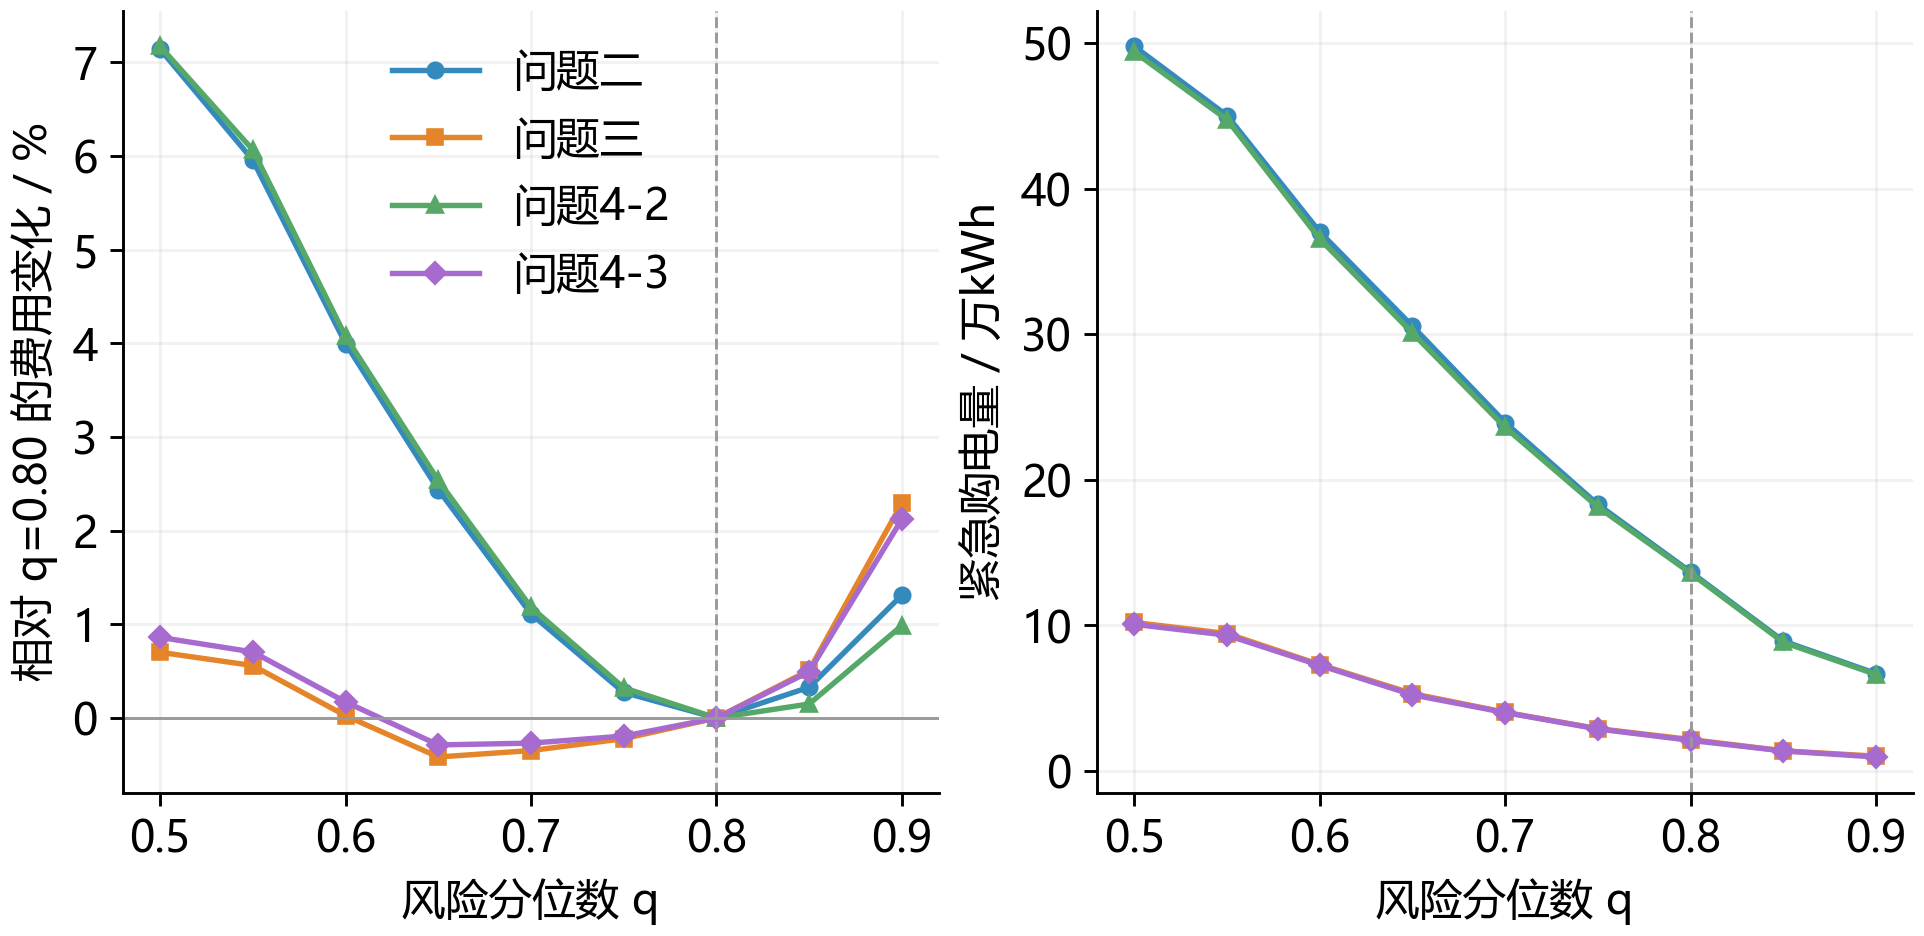
\includegraphics[width=0.90\textwidth,height=0.55\textheight,keepaspectratio]{fig12.png}
\caption*{图12 分位数对总费用及紧急购电量的影响（正式期334天）}
\end{figure}

图12把表 12 的总费用按各问题 $q=0.80$ 的基线归一化，并展示紧急购电量。四问紧急购电量随分位数升高而下降，但总费用并不单调下降；问题三与问题 4-3 的扫描最低点出现在 $q=0.65$，问题二与问题 4-2 出现在 $q=0.80$。该图仅呈现冻结扫描结果，不用于重新选择正式参数。

扫描结果呈现一个清晰的权衡。分位数提高会增大储备、抬高日末储电量下限，从而压缩谷段的低价充电空间，使计划购电费上升；但储备增大同时减少紧急购电，而紧急购电价格是同时段电价的 5 倍，其边际成本远高于储备带来的机会成本。两者相抵，费用曲线在中间某个档位取到最低。

具体数值为：问题二与问题 4-2 的最低点出现在 $q=0.80$，分别为 13,864,639.36 元与 14,595,194.94 元；问题三与问题 4-3 的最低点出现在 $q=0.65$，分别为 13,383,133.11 元与 14,117,475.69 元，比各自的 $q=0.80$ 结果低 55,911.26 元与 40,650.05 元。四者的紧急购电天数在 $q$ 从 0.50 升至 0.90 的过程中分别由 331、280、328、276 天降至 111、109、109、109 天，说明储备的提升确实在持续压缩紧急购电，只是压缩到一定程度后其费用收益已不足以抵偿充电机会成本的增加。

问题三与问题 4-3 的扫描最低点低于问题二与问题 4-2，说明同一分位数在四个子问题上的实际效果并不相同。本文不对这一差别给出机制性解释：执行器并不接收储备量 $R$，$R$ 只通过计划层给出的承诺量 $x_{d,i}^{\mathrm{exec}}$ 间接影响执行结果（见式(34)、(35)），因此无法把这一差别直接归因于"储备压缩了贪心执行的放电空间"。可以确证的只有扫描表本身所呈现的形态：在本文扫描的九个档位上，四个子问题都表现为费用先降后升、紧急购电天数单调下降，只是最低点所在的档位不同。这提示"统一取 0.80"对四个子问题并非同等合适；本文保留事前的统一取值以保证四个子问题可比，把分档设置列为改进方向（见 7.2 节）。

三点限定必须随表 12 一起给出。第一，四个子问题的最优档位分别出现在扫描序列的第 7 档与第 4 档，是事后的观察结果，"0.65 更好"只在本文扫描的这九个档位内成立，不能排除更细的步长下最低点落在别处。第二，$q=0.65$ 相对 $0.80$ 的改进幅度（问题三 55,911.26 元，占总费用的 0.42\%）不足以支撑改动正式交付方案的取值——正式结果仍以 $q=0.80$ 为准。第三，分位数 $q$ 控制的是历史残差的覆盖比例，它\textbf{不等于}紧急购电不发生概率，也不等于供电可靠性指标：残差的经验覆盖率与"当天不启用紧急购电"之间没有一一对应关系，见表 12 中覆盖率由 0.751 升至 0.901 时紧急购电天数仅由 141 天降至 109 天。因此本文只把 $q$ 作为控制储备水平的参数，不把它解释为可靠性保证。

\needspace{3\baselineskip}\subsection*{6.4 结论的适用边界}

综合 6.1—6.3 的检验，本文结论的适用范围可归纳为以下几条。

在评价期上，正式结论以 2025-02-01 至 2025-12-31 的 334 天为准，四个子问题的年末储电量均收口到 6000 kWh。自然年 365 天的口径在 5.2.4、5.3.5 节中作为对照给出，其中 5.3.5 节已说明"关闭 6:00"的收益在自然年口径下反号，故该条建议只限正式期。

在结算口径上，多版承诺的合成方式采用项目自定的解释口径。题面给出了基准费与调整费的方向性费率，但没有给出多版承诺如何组合为最终基准量的官方解释文件；本文按 第三章假设（5）声明的口径实现，四个子问题在同一口径下可比。若官方另有解释，第 5.3、5.4 节的费用数字需要按新口径重算，但模型的决策结构与执行逻辑不受影响。

在方法上，本文的策略是"物理可行、阶段可解、费用可核验"的策略，而不是已证最优的策略。6.2 节的对照阶梯给出的是信息价值的量级，不是最优性证明；6.3 节的扫描给出的是参数敏感性，不是参数最优性证明。本文不放宽对这几点的表述。

在数据上，本文没有获得任何气象观测数据，对结果的季节性差异只做描述性说明（光伏出力的季节差异、负荷的季节差异），不把月度差异归因于具体的降温负荷或最冷周次，也不引用未经核实的气象数值。

\needspace{4\baselineskip}\section*{七、模型评价与改进}

\needspace{3\baselineskip}\subsection*{7.1 模型的优点}

\textbf{物理一致}。全部四个子问题的解都逐时段满足功率平衡、储电量递推与设备功率约束。52,560 个时段的核验显示按每段电量折算的平衡最大残差为 $2.27\times10^{-13}$ kWh，储电量越界、功率越界、同时充放电与反向购电的时段数全部为 0，说明模型给出的调度指令可以直接执行，不存在只满足总量而不满足逐时段的"纸面方案"。

\textbf{阶段模型可解}。问题一、问题二的计划层是标准线性规划，问题三、问题 4-3 的单阶段计划层是含 $n$ 个 0-1 变量的小规模混合整数线性规划，规模随时段数线性增长，不随评价期长度变化。0-1 变量只出现在历史最小承诺的分支选择上，数量与时段数同阶；两条线性化约束中，第一条以历史最小承诺 $m$ 作紧系数，第二条取固定常数 $M=6.0\times10^{5}$ kW 作松弛量，分支定界的规模可控。

\textbf{费用可核验}。结算费用不是事后估算，而是按式(26)的链式增量逐阶段累加，并与逐日总费用做恒等式核验，全部 365 天的偏差小于 $10^{-5}$ 元。式(26)的分段形态在 $z=p$ 与 $z=m$ 两处连续，可用手算逐段复核。

\textbf{实验可追溯}。全部数字来自同一套代码、同一份冻结数据，四个子问题使用同一套参数，未做逐问题的单独调参。消融实验（表9）与灵敏度扫描（表 12）都由同一次批量实验生成，表 11 的四个档位也由同一套代码回放得到。

\needspace{3\baselineskip}\subsection*{7.2 模型的缺点与改进方向}

\textbf{跨年推广性未经检验}。本文全部结论建立在 2025 年这一年的数据上，年末收口到 6000 kWh 的做法在多年连续运行下是否仍然合适、跨年储电量如何摊销，本文没有数据可以检验，也没有做多年滚动实验。若要推广到多年，需要引入年末储电量的残值曲线并重新标定。

\textbf{发布时点的启用配置仍可优化}。5.3.5 节说明 6:00 的边际价值在完整配置下已转为负值，但这一结论依赖评价期的选取（自然年口径下反号）。更稳健的做法是把"启用哪些时点"本身作为决策变量，在跨口径的稳健性目标下选择，而不是固定四个时点全开或按单一口径裁剪。

\textbf{统一分位数可能不适合不同发布窗口}。6.3 节显示问题三、问题 4-3 的扫描最低点在 0.65、问题二、问题 4-2 在 0.80。四个发布时点的残差统计窗口长度不同（143、108、72、36 个时段），同一分位数在不同窗口下的实际储备水平差异很大。按窗口长度分别设定分位数是自然的改进方向，但需要额外的验证数据来避免过拟合。

\textbf{预测与执行的协调可以改进}。问题三、问题 4-3 的执行层是无前视的贪心规则，式(34)、(35)在每个时段只做局部最优判断；问题二、问题 4-2 使用 36 时段滚动优化但也只执行第一步。把执行层的前视窗口与发布时刻对齐（例如在 6:00 之后用覆盖至下次发布时刻的短窗优化），有可能同时改善两者的表现，本文未做该实验。

\textbf{外网容量上限与紧急购电的固定成本未纳入}。题目未对购电功率设上限，本文也未假设紧急购电存在启动固定成本。若实际运行中存在线路容量约束或紧急采购的最小起订量，需要在式(19)、(20)中增加相应约束，本文把它们列为扩展方向而不在当前模型中虚构这些参数。

\clearpage\begin{center}\heiti\bfseries\zihao{4}参考文献\end{center}

{\footnotesize\noindent\hangindent=0.65cm\hangafter=1 [1] 国家市场监督管理总局, 国家标准化管理委员会. 光伏发电系统接入配电网技术规定: GB/T 29319—2024[S]. 2024.\par}

{\footnotesize\noindent\hangindent=0.65cm\hangafter=1 [2] PACAUD F, CARPENTIER P, CHANCELIER J P, et al. Stochastic optimal control of a domestic microgrid equipped with solar panel and battery[EB/OL]. (2018-01-19)[2026-09-13]. \url{https://arxiv.org/abs/1801.06479}.\par}

{\footnotesize\noindent\hangindent=0.65cm\hangafter=1 [3] 胡运权, 郭耀煌. 运筹学教程[M]. 5版. 北京: 清华大学出版社, 2018.\par}

{\footnotesize\noindent\hangindent=0.65cm\hangafter=1 [4] 姜启源, 谢金星, 叶俊. 数学模型[M]. 5版. 北京: 高等教育出版社, 2018.\par}

{\footnotesize\noindent\hangindent=0.65cm\hangafter=1 [5] 国家发展和改革委员会. 关于进一步完善分时电价机制的通知: 发改价格〔2021〕1093号[A]. 成文日期 2021-07-26, 发布日期 2021-07-29.\par}

{\footnotesize\noindent\hangindent=0.65cm\hangafter=1 [6] KE G, MENG Q, FINLEY T, et al. LightGBM: A Highly Efficient Gradient Boosting Decision Tree[C]//Advances in Neural Information Processing Systems 30. 2017.\par}

{\footnotesize\noindent\hangindent=0.65cm\hangafter=1 [7] IHEANETU K J. Solar Photovoltaic Power Forecasting: A Review[J]. Sustainability, 2022, 14(24): 17005. DOI:10.3390/su142417005.\par}

{\footnotesize\noindent\hangindent=0.65cm\hangafter=1 [8] ROCKAFELLAR R T, URYASEV S. Optimization of conditional value-at-risk[J]. Journal of Risk, 2000, 2(3): 21-41.\par}

{\footnotesize\noindent\hangindent=0.65cm\hangafter=1 [9] MORSTYN T, HREDZAK B, AGUILERA R P, et al. Model Predictive Control for Distributed Microgrid Battery Energy Storage Systems[EB/OL]. (2017-02-15)[2026-09-13]. \url{https://arxiv.org/abs/1702.04699}.\par}

{\footnotesize\noindent\hangindent=0.65cm\hangafter=1 [10] PERERA M, DE HOOG J, BANDARA K, et al. Multi-Resolution, Multi-Horizon Distributed Solar PV Power Forecasting with Forecast Combinations[EB/OL]. (2022-06-22)[2026-09-13]. \url{https://arxiv.org/abs/2206.10795}.\par}

\needspace{4\baselineskip}\section*{AI 工具使用声明}

本队在本题的完成过程中使用了人工智能辅助工具，使用范围为：辅助核对代码与结果文件中的数值一致性、辅助排版论文的公式与表格、辅助整理文献与文字表达。全部模型建立、算法设计、程序编写、参数选择与结果分析由队员完成，人工智能工具未参与产生任何实验数据或结论。所有出现在论文中的数值均来自本队程序的运行输出，并已与冻结结果文件逐项核对。

具体的使用记录（工具名称、使用日期、对话要点）由队长在提交前按竞赛要求补充并签署。本处不代填未经确认的记录。

\needspace{4\baselineskip}\section*{附录}

\needspace{3\baselineskip}\subsection*{附录 A 支撑材料文件列表}

见随论文提交的支撑材料目录说明文件。核心内容包括：共享模型与求解代码、四个（子）问题的一键运行脚本、全年逐时段结果（物理轴 10 分钟粒度与计划轴粒度各一份）、冻结数值汇总文件、物理可行性核验与结算恒等式核验的原始输出。

\needspace{3\baselineskip}\subsection*{附录 B 关键数据表}

题目要求的三张指定日期表（表 1、表 2、表 3 口径）在四个子问题下各有一份完整结果，分别对应正文表 7、表 8、表10。全年逐日与逐时段明细以 CSV 形式随支撑材料提交，不在正文中展开。

\needspace{3\baselineskip}\subsection*{附录 C 文献与新增图表的核查说明}

本轮新增五项文献的可下载 PDF 已随支撑材料提供，分别支持 LightGBM、微网储能 MPC、光伏预测组合、微网不确定性控制及光伏预测背景。它们不证明本文特定融合系数、路径最小承诺结算假设或最优分位数。MPC、光伏预测组合及家庭微网不确定性控制三项按实际下载的作者稿著录；文献\textsuperscript{[10]}的正式论文 DOI 为 10.1016/j.eswa.2022.117690。

新增两图均由既有冻结数据生成，未重新拟合预测或重跑优化。光伏来源对照使用共享预测缓存、附件 3 对齐规则及正式融合输出；风险费用图使用表 D 的334天扫描。对应绘图数据位于 \_build/figure\_data，可逐点核查。

\end{document}
